\documentclass[a4paper]{article}
\usepackage{cmap}
\usepackage[utf8]{inputenc}
\usepackage[russian]{babel}
\usepackage{float}
\usepackage[justification=centering]{caption}
\usepackage{graphicx}
\usepackage{amsmath}
\usepackage{amssymb}
\usepackage{amsthm}
\usepackage{indentfirst}
\usepackage[unicode, pdfborder = {0 0 0}, colorlinks, linkcolor = black]{hyperref}
\usepackage[raggedright]{titlesec}
\usepackage{mathtools}
\usepackage{chngcntr}


\counterwithin{figure}{section}

 
\DeclarePairedDelimiter\ceil{\lceil}{\rceil}
\DeclarePairedDelimiter\floor{\lfloor}{\rfloor}


\titleformat{\chapter}[block]
  {\normalfont\huge\bfseries}{\thechapter}{20pt}{}
\titlespacing*{\chapter}
  {0pt}{20pt}{20pt}

\setcounter{tocdepth}{5}
\setcounter{secnumdepth}{5}


\parindent = 7mm
\oddsidemargin = 5mm
\topmargin = -10mm
\textheight = 240mm
\textwidth = 165mm
\linespread{1.5}

\captionsetup{labelsep=period}

\renewcommand{\small}{\fontsize{12}{14.5pt}\selectfont}
\renewcommand{\normalsize}{\fontsize{14}{16pt}\selectfont}
\renewcommand{\large}{\fontsize{17}{20pt}\selectfont}
\renewcommand{\Large}{\fontsize{20}{25pt}\selectfont}
\renewcommand{\LARGE}{\fontsize{25}{30pt}\selectfont}
\renewcommand\qedsymbol{$\blacksquare$}

\newtheorem{theorem}{Теорема}[section]
\theoremstyle{definition}
\newtheorem{statement}{Утверждение}[section]
\newtheorem{definition}{Определение}[section]
\newtheorem{example}{Пример}[section]

\newenvironment{Proof}
    {{\bf \flushleft{Доказательство.} \\}}
    {\hfill$\scriptstyle\blacksquare$}


\newcounter{qcounter}


\begin{document}
\normalsize

    \thispagestyle{empty}
    \begin{titlepage}
    \begin{center}


    \vfill
    МИНОБРНАУКИ РОССИИ\\
    \vspace*{0.3cm}
    Федеральное государственное автономное образовательное\\
    учреждение высшего образования\\
    «Южный федеральный университет»\\
    \vspace*{0.3cm}
    Институт математики, механики и компьютерных наук им.\\
    И.И.Воровича\\
    Кафедра алгебры и дискретной математики
    \vfill


    \bigskip


    {\large\bf Ковалев~Никита~Евгеньевич}
    \vfill
    {\large\bf ВОССТАНОВЛЕНИЕ ЦИКЛИЧЕСКИ\\СМАЗАННЫХ ИЗОБРАЖЕНИЙ\\
               С ВЫРОЖДЕННЫМ СМАЗОМ}

\fontsize{14}{16pt}\selectfont

    \vfill
    ВЫПУСКНАЯ КВАЛИФИКАЦИОННАЯ\\ РАБОТА БАКАЛАВРА\\
    по направлению 01.03.02 — Прикладная математика и информатика
    \vfill

    {\bf Научный руководитель~---\\
         доц., к.ф.-м.н. Козак Анатолий Всеволодович}



    \vfill

    \end{center}

    \bigskip

    \begin{center}
        Ростов-на-Дону~---~2018
    \end{center}

    \end{titlepage}

%-------------------------------------
    \tableofcontents
    \newpage
%-------------------------------------


    \section*{Введение}
    \addcontentsline{toc}{section}{Введение}


    С появлением фотокамер человечество получило инструмент, позволяющий сохранять информацию о любых видимых объектах окружающей среды. Но снимки, получаемые с помощью фотокамеры, не всегда хорошего качества по многим причинам. Безусловно, фотокамеры совершенствуются со временем, и сейчас они способны устранять многие искажения еще при обработке и сохранении снимка, однако, особенно при тяжелых условиях съемки, зачастую фотографии не отражают столько информации, сколько необходимо. С развитием техники появились инструменты для работы с искаженными фото, а ЭВМ обрели вычислительную мощность, достаточную для обработки фото высокого разрешения за достаточно быстрое время. Также из всех возможных искажений выделили некоторые классы явлений, с которыми есть возможность работать в рамках определенных методов. Одним из таких негативных эффектов является смаз (\cite{blur_def}).


    В данной работе рассматривается горизонтальный циклический смаз. Он возникает при съемке местности с помощью вращающейся камеры при создании панорамных снимков. При смазе такого типа каждый пиксель смазанного изображения это есть среднее арифметическое нескольких соседствующих по горизонтали пикселей исходного, ``правильного'' изображения. Таким образом, чем больше число смаза, тем больше исходных пикселей содержится в каждом пикселе смазанного фото, и информация о них лежит в младших разрядах, поэтому при оцифровке (сохранении) изображения часть информации теряется. Вследствие этого большое влияние на потенциальное качество восстановления изображения оказывает количество бит на пиксел при оцифровке, так как точность округления выше для 16-битных изображений, нежели для 8-битных. А поскольку задача актуальна для таких областей, как военная разведка, картография, геодезия, моделирование объектов местности и аналогичных, то отснять материал заново зачастую невозможно. Поэтому задача максимально точного восстановления искаженных снимков приобретает важный характер.


    В большинстве методов восстановления смаза используется подход с ядром преобразования (\cite{kernel1}-\cite{kernel2}), то есть по входному изображению находится ядро свертки, а затем вычисляется обратная свертка (деконволюция). Поскольку в данной работе исследуется горизонтальный смаз с известным видом общей матрицы, то целесообразно использовать представление смаза как обычного матричного перемножения (как, например, в \cite{model_proc} и \cite{cond}).


    По причине того, что данная задача требует выполнения перемножений матриц большого размера, а также работы с матрицами комплексных чисел, необходимо выбрать наиболее эффективный язык для реализации методов. Таковым, определенно, является MATLAB (сокр. от MATrix LABoratory; \cite{matlab}), и, так как лицензированная MATLAB-среда имеется в дисплейных классах Института математики, механики и компьютерных наук имени И.И. Воровича, то я остановился именно на ней. Это позволило добиться действительно быстрой работы описаннных в работе методов.


    Стоит отметить, что на протяжении всего учебного года мы вместе с другими студентами периодически обсуждали промежуточные результаты наших работ, а также различные тенденции в ведущих областях исследований по нашим темам. В процессе таких дискуссий рождалось множество идей для продолжения наших исследований, в том числе таким образом был придуман один из важнейших аспектов второго метода из описанных в данной работе.


%-------------------------------------
    \newpage
%-------------------------------------

    \section{Вспомогательные понятия}


    Введем некоторые обозначения и базовые понятия, которые будут использоваться в дальнейшем.


    \begin{definition}
    \label{blur}
    При \emph{горизонтальном циклическом смазе} каждый пиксель изображения это среднее нескольких пикселей исходного/восстановленного изображения. Само фото в данном случае представляет собой цилиндрическую панораму, именно поэтому смаз называют циклическим.
    \end{definition}


    Чтобы смоделировать \emph{горизонтальный циклический смаз} (далее - \emph{смаз}) необходимо умножить изображение на соответствующую матрицу смаза справа. Поэтому необходимо задать матрицу, его определяющую. Так как мы знаем, что в смазанном изображении каждый пиксель это среднее нескольких пикселей исходного, и смаз циклический (то есть края изображения влияют друг на друга), то матрица будет действовать на все изображение одинаково и каждый столбец будет состоять из $k$ чисел, равных $\frac{1}{k}$ (именно при таких числах мы получим среднее арифметическое $k$ пикселей исходного изображения). Также нужно учесть, что по мере движения по изображению горизонтально пиксели, которые учитываются для получения текущего пиксела, должны сдвигаться в том же направлении. Это означает, что ненулевые числа в столбце будут циклически сдвигаться на единицу по сравнению с соседним. Учитывая вышесказанное, определим матрицу смаза.


\newpage
    \begin{definition}
    \label{blur matrix}
	\emph{Матрицей горизонтального циклического смаза} (далее - \emph{матрицей смаза}) изображения ширины $n$ на $k$ пикселей называется матрица $C(n, k) \in M_n$ вида
    $$
    C(n, k) = \frac{1}{k}\begin{pmatrix}
          \overbrace{1 \hspace*{2mm} \ldots \hspace*{2mm} 1 \hspace*{2mm} 1}^{k} \hspace*{2mm} 0 \hspace*{2mm} \ldots \hspace*{2mm} 0 \\
          0 \hspace*{2mm} 1 \hspace*{2mm} \ldots \hspace*{2mm} 1 \hspace*{2mm} 1 \hspace*{2mm} \ldots \hspace*{2mm} 0 \\
          \ldots \hspace*{2mm} \ddots \hspace*{2mm} \ldots \hspace*{2mm} \ddots \hspace*{2mm} \ldots \\
          1 \hspace*{2mm} \ldots \hspace*{2mm} 0 \hspace*{2mm} 1 \hspace*{2mm} 1 \hspace*{2mm} \ldots \hspace*{2mm} 1 \\
          \ldots \hspace*{2mm} \ddots \hspace*{2mm} \ldots \hspace*{2mm} \ddots \hspace*{2mm} \ldots\\
          \underbrace{1 \hspace*{2mm} \ldots \hspace*{2mm} 1}_{k-1} \hspace*{2mm} 0 \hspace*{2mm} 0 \hspace*{2mm} \ldots \hspace*{2mm} 1
        \end{pmatrix}
    $$
    \end{definition}


    В дальнейшем будем отождествлять понятие матрицы смаза и обозначения $C(n, k)$ и просто $C$ (если параметры $n$ и $k$ ясны из контекста).
\vspace{0.3cm}


    \begin{statement}[об обратимости матрицы смаза]
    \label{inverse}
	Матрица смаза обратима тогда и только тогда, когда НОД$(n, k) = 1$ (\cite{cond}).
    \end{statement}


    Следствием Утверждения \ref{inverse} является, среди прочего, большее количество изображений с вырожденным смазом, нежели с невырожденным, что лишний раз подтверждает актуальность поставленной задачи.


    \begin{statement}[о представлении матрицы смаза]
    \label{fourier}
        Матрица смаза всегда представима в виде $FDF^{-1}$, где $F$ и $F^{-1}$ - соответственно прямое и обратное дискретные преобразования Фурье (\cite{fft_def}), а $D$ - диагональная матрица, причем на диагонали - собственные значения матрицы $C$, и такое представление единственно.

    \end{statement}


\newpage
    \begin{example}
    Приведем пример изображений и их смазанные варианты.

\hspace*{-\parindent}
\begin{minipage}{80mm}
  \begin{figure}[H]
            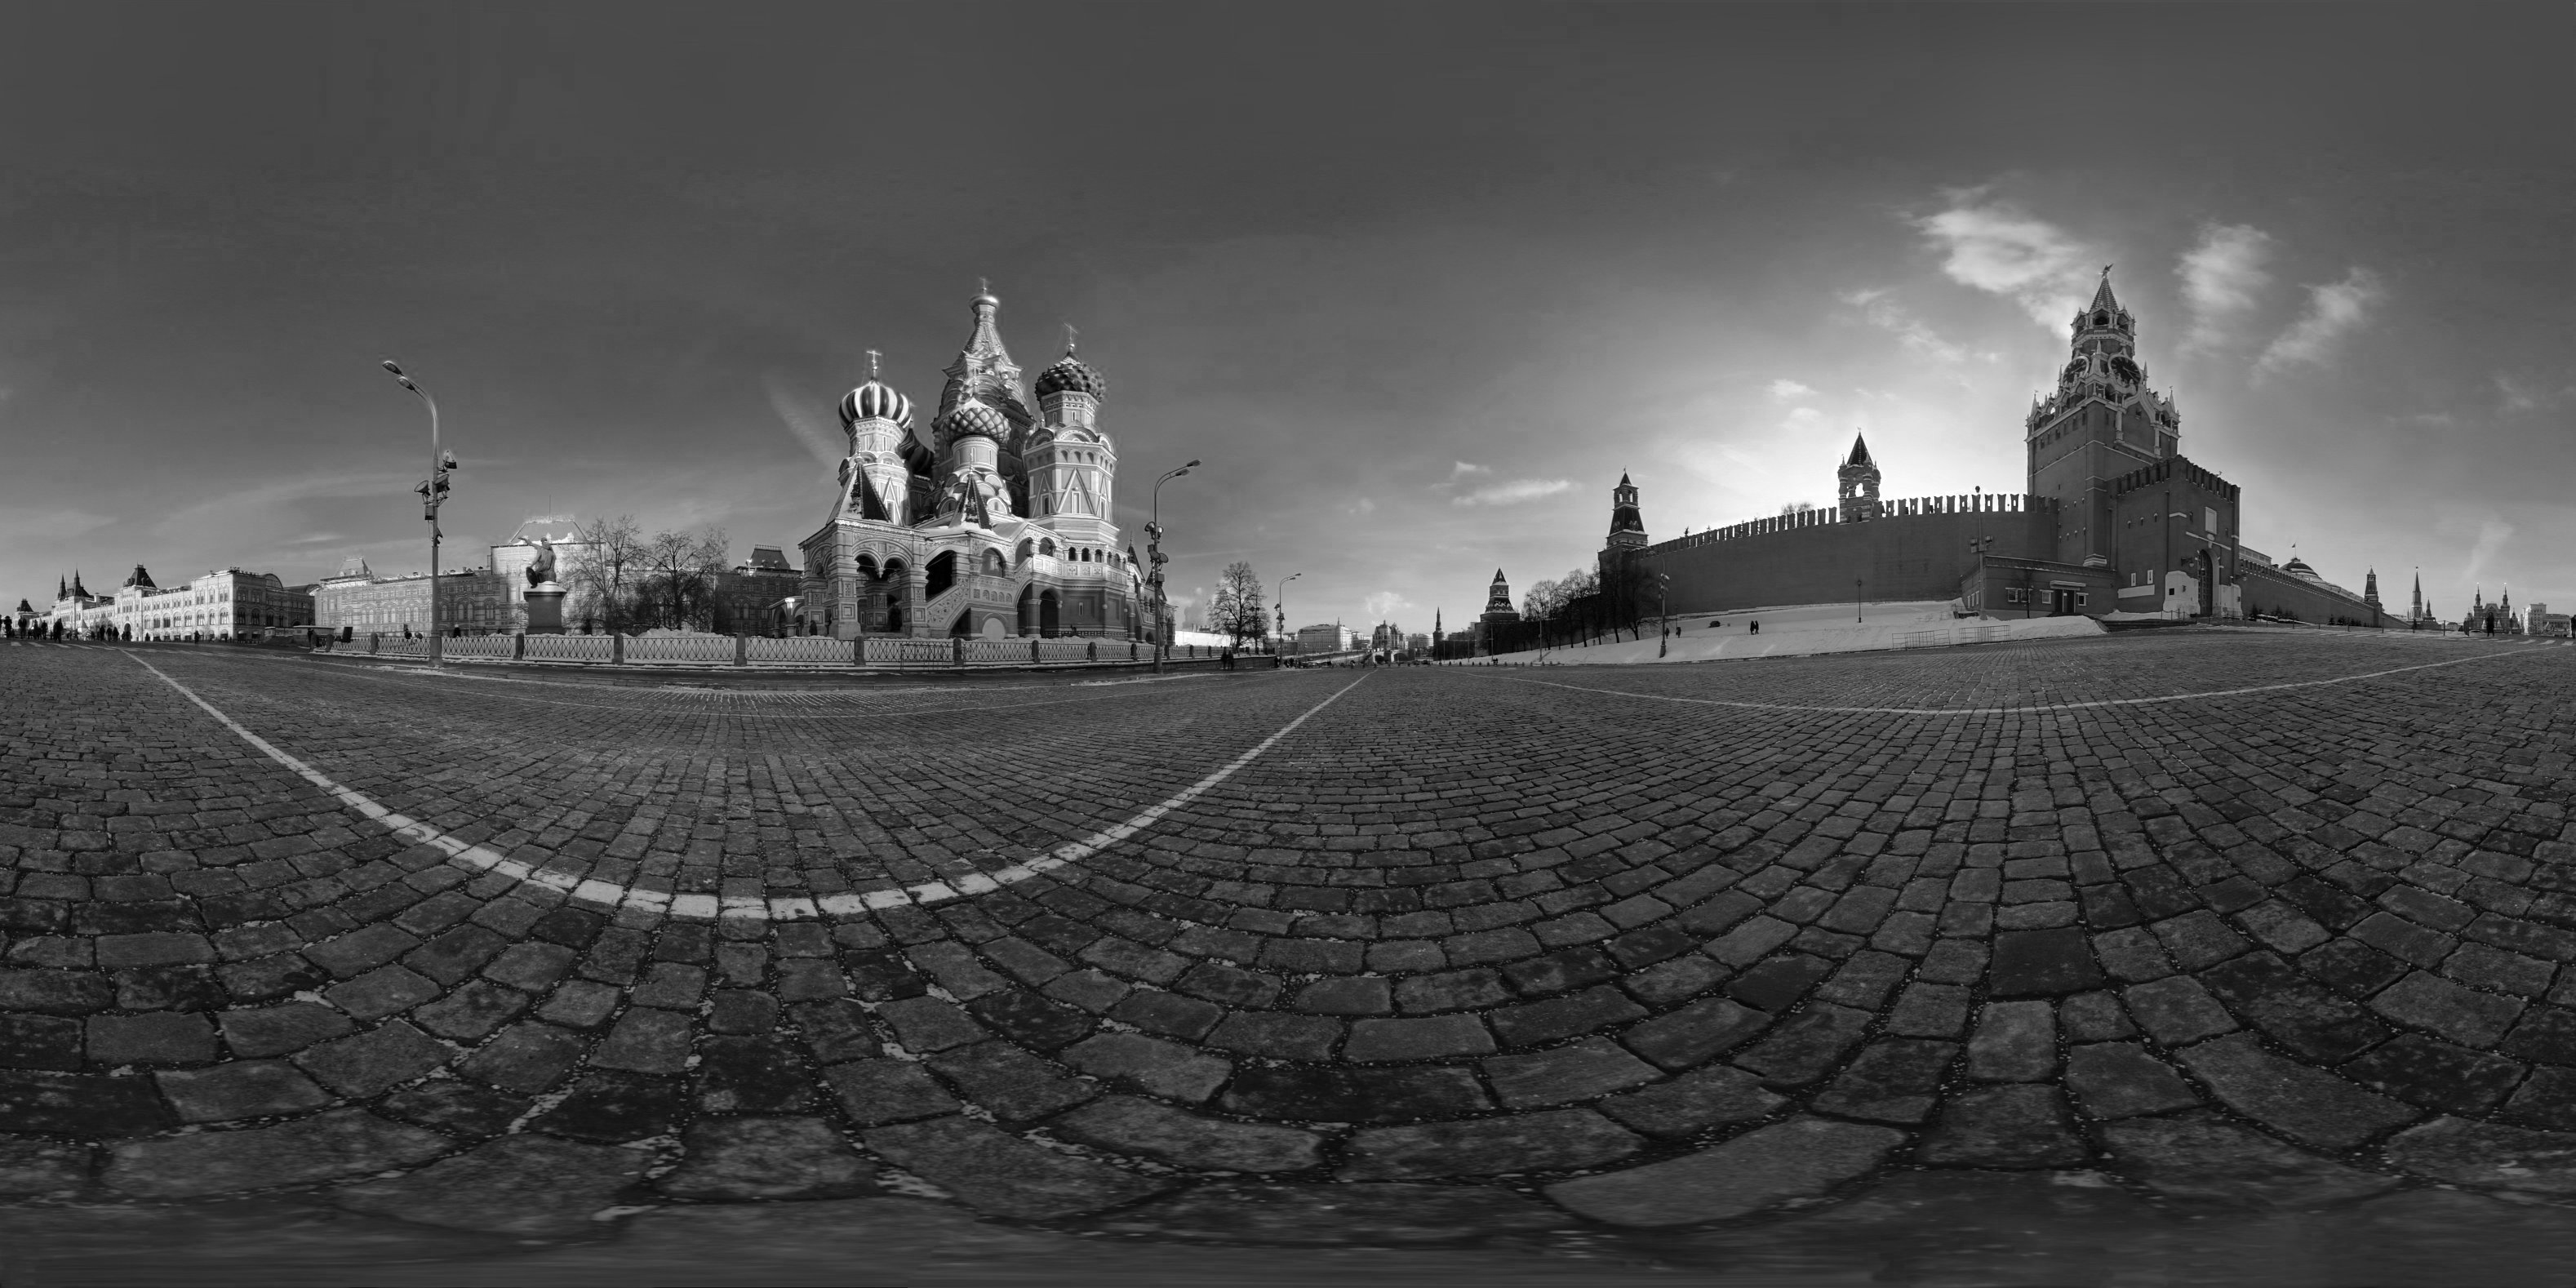
\includegraphics[scale=0.07]{G:/Study/tex_diploma/Pictures/fig2.png}
            \label{Fig2}
            \caption[Исходное изображение]{Исходное изображение}
        \end{figure}
\end{minipage}
\begin{minipage}{80mm}
    \begin{figure}[H]
            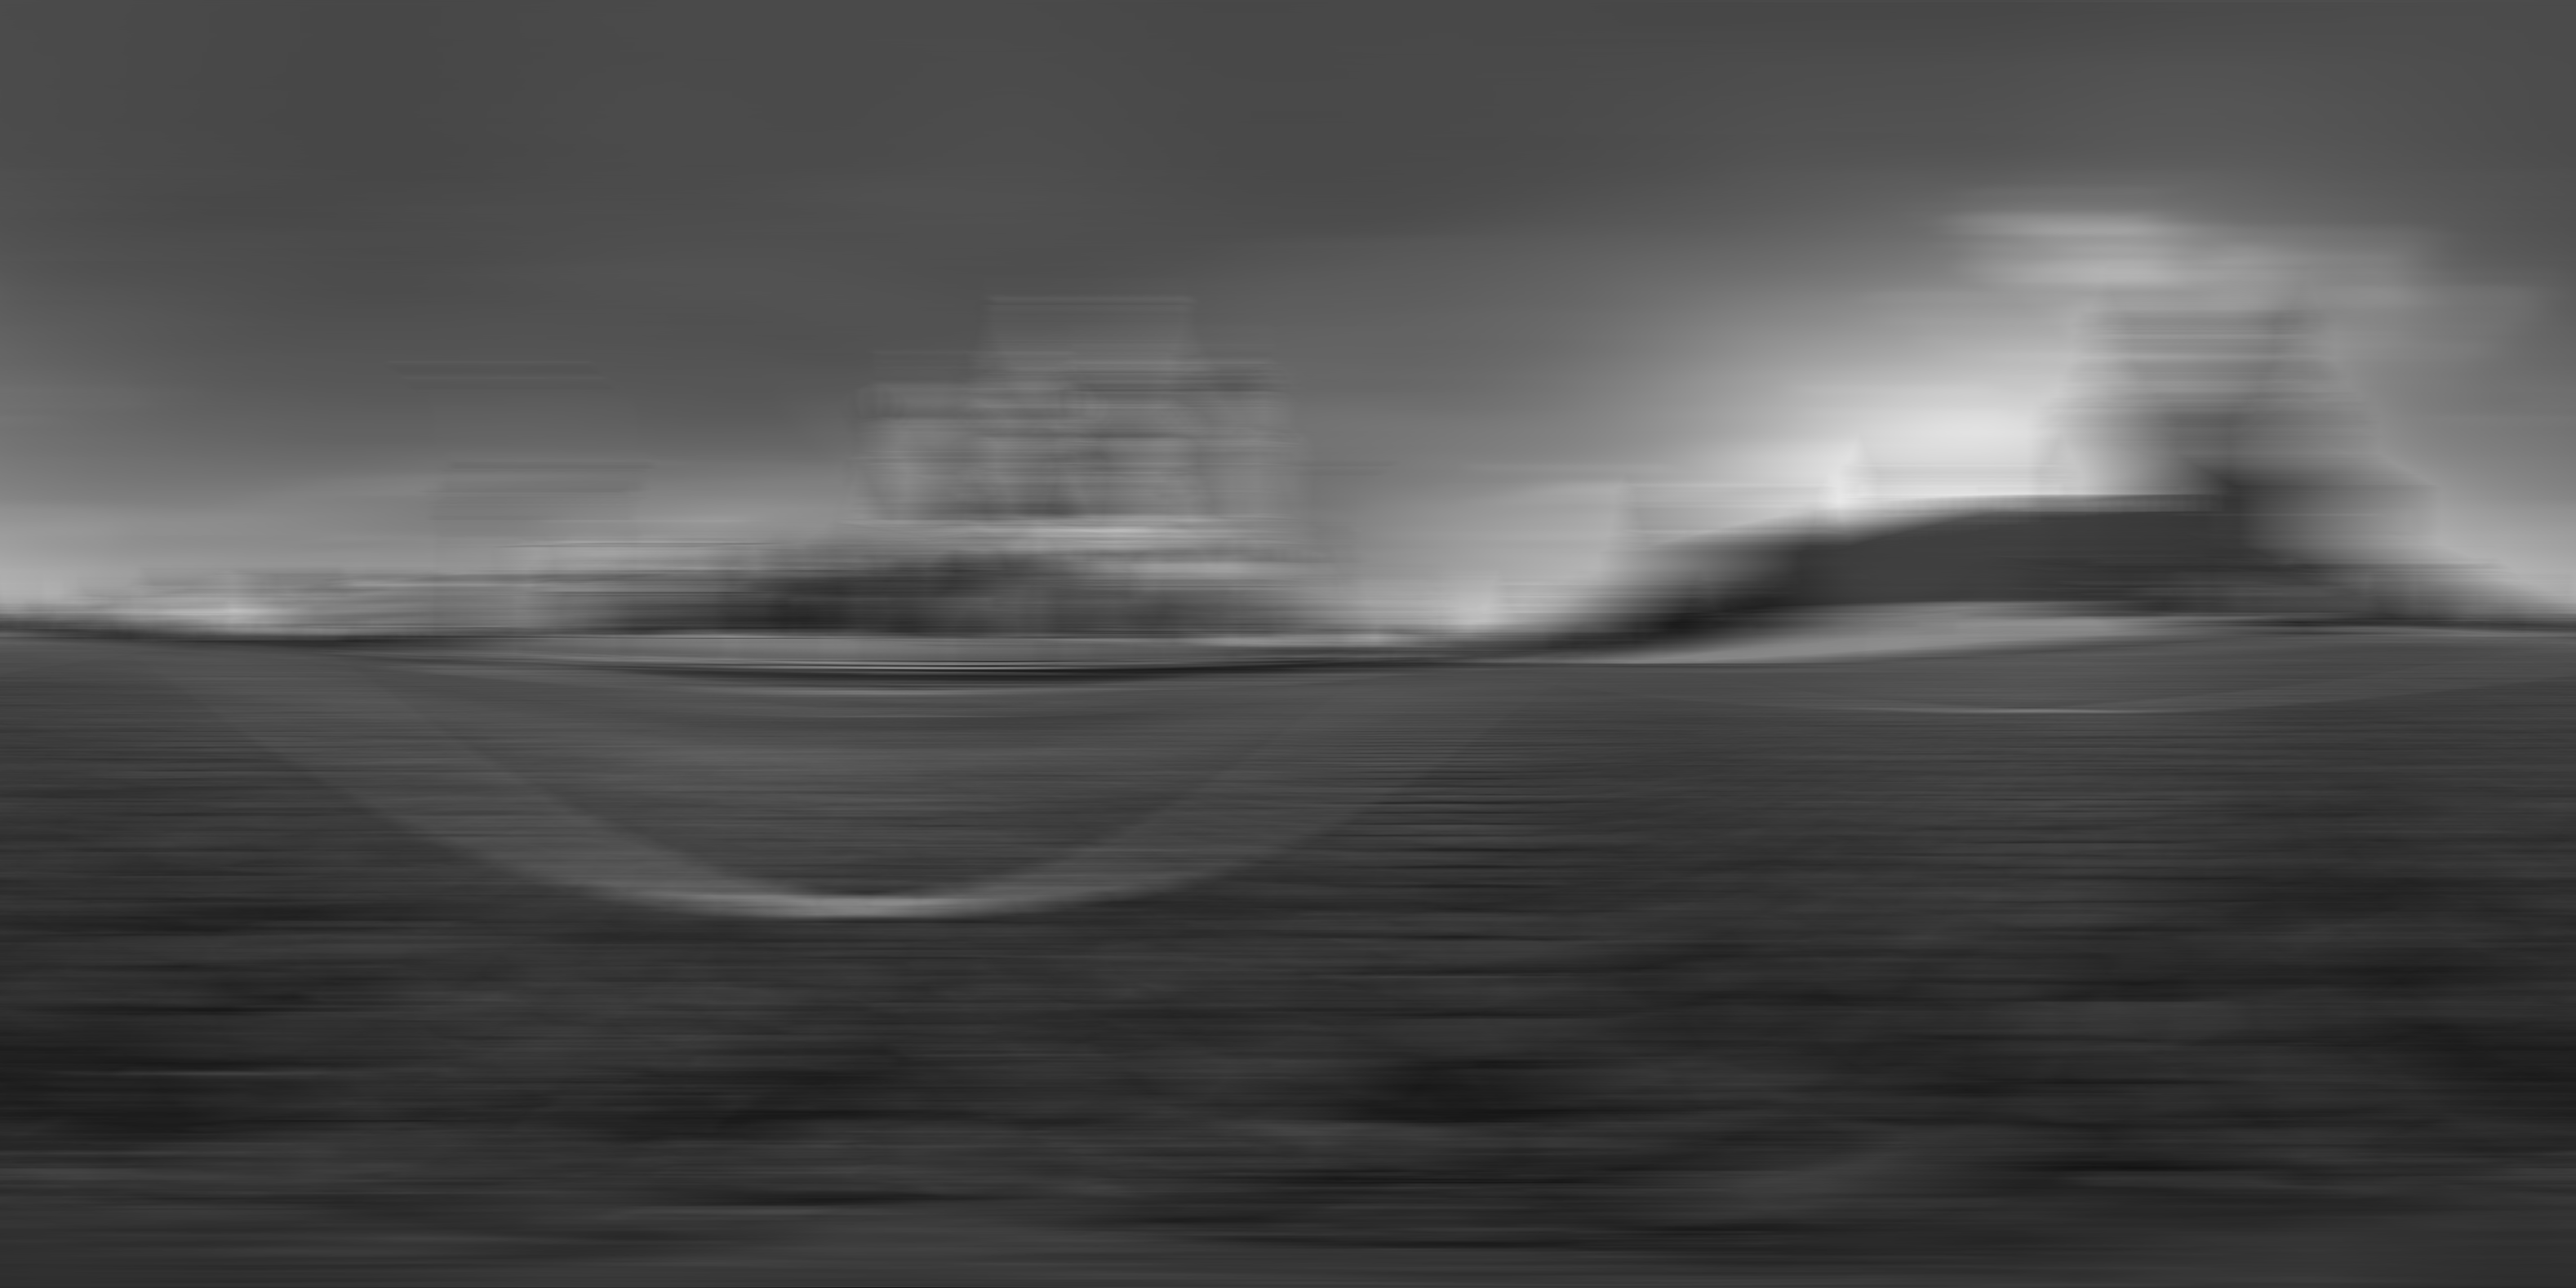
\includegraphics[scale=0.07]{G:/Study/tex_diploma/Pictures/fig1.png}
            \label{Fig1}
            \caption[Смаз при $k$ = 248]{Смаз при $k$ = 248}
        \end{figure}
\end{minipage}
\hfill
\vspace*{3mm}


Это изображение хорошо для исследования реальных ситуаций, так как оно является панорамным, то есть левая часть фото продолжает правую. Тем не менее, на самом деле, для качественного изучения результатов достаточно взять любое изображение.

\hspace*{-\parindent}
\begin{minipage}{80mm}
  \begin{figure}[H]
            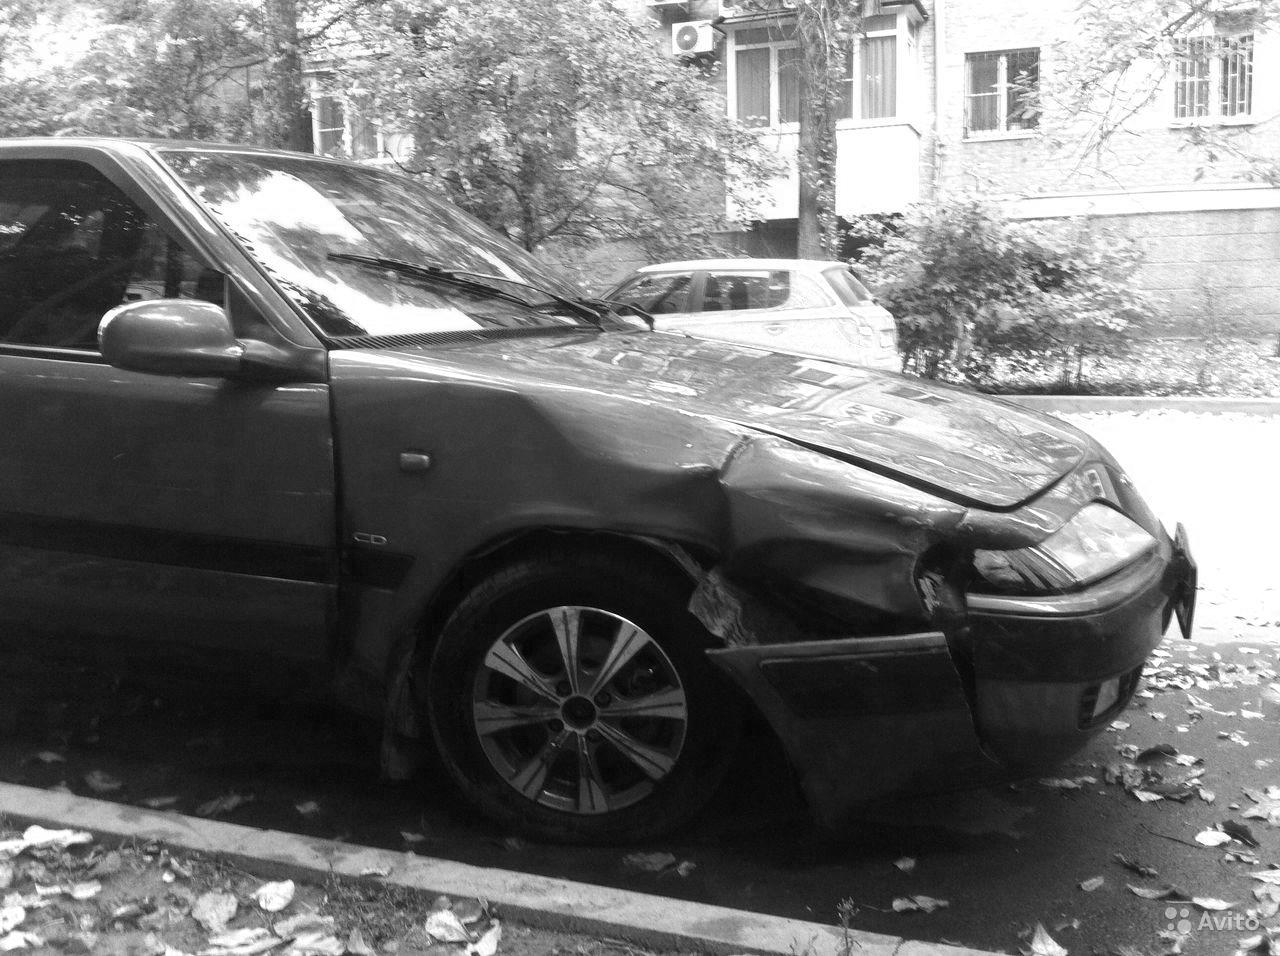
\includegraphics[scale=0.16]{G:/Study/tex_diploma/Pictures/8.png}
            \label{Fig_8}
            \caption[Исходное изображение]{Исходное изображение}
        \end{figure}
\end{minipage}
\begin{minipage}{80mm}
    \begin{figure}[H]
            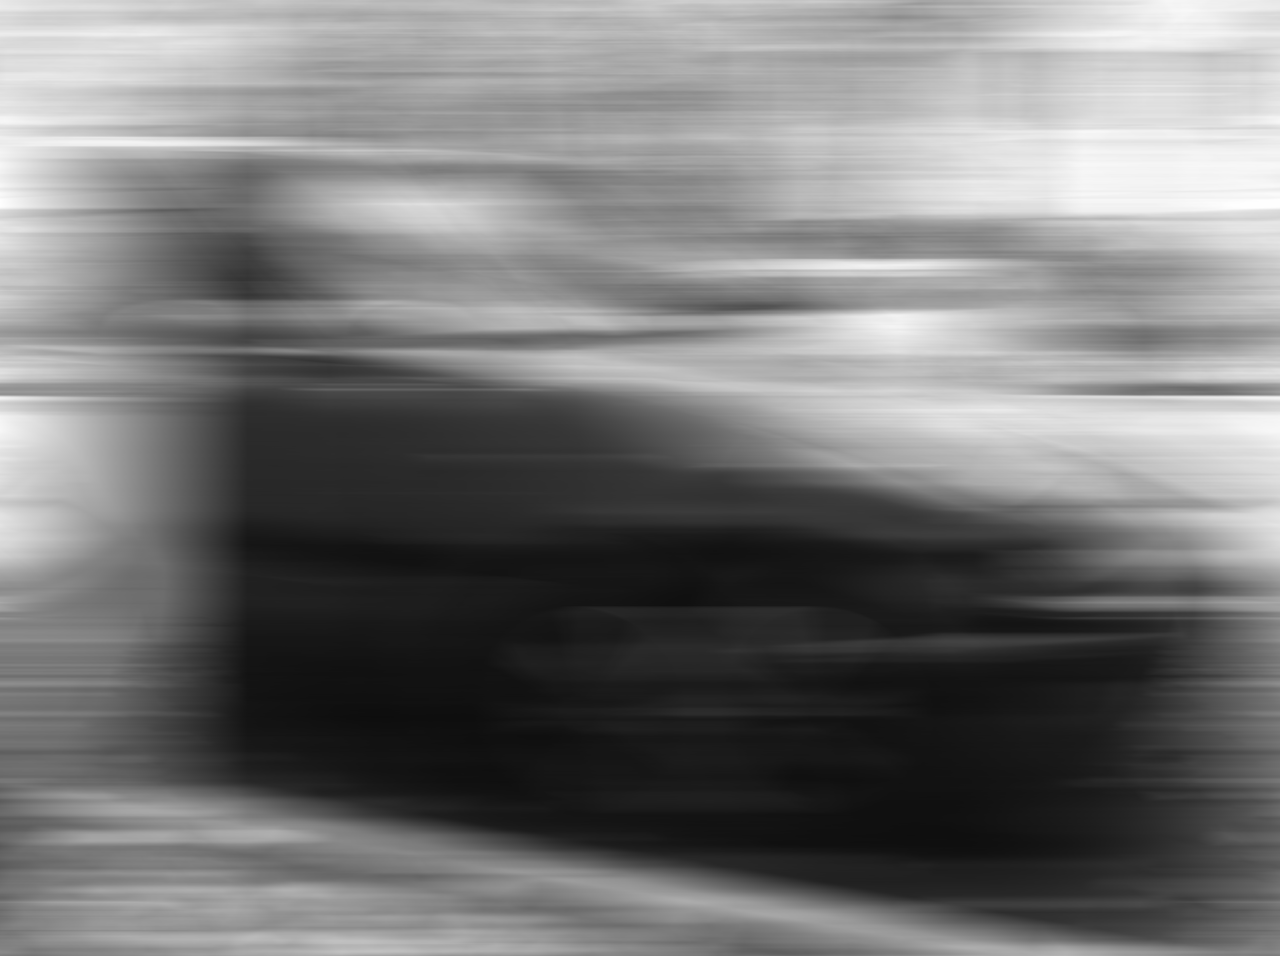
\includegraphics[scale=0.16]{G:/Study/tex_diploma/Pictures/8_smaz248.png}
            \label{Fig_8s}
            \caption[Смаз при $k$ = 248]{Смаз при $k$ = 248}
        \end{figure}
\end{minipage}
\hfill

    \end{example}

%--------------------------------------
    \newpage
%-------------------------------------


    \section{Метод предобработки в случае большого числа смаза}


    В первой части пойдет речь о методе, который эффективен только для восстановления 16-битных изображений, поскольку данный подход использует обычное восстановление для невырожденного случая. Для 8-битного изображения даже при высокой (в том числе идеальной) математической точности на восстановленном фото появляется шум (\cite{noise}), так как даже в невырожденном случае число обусловленности матрицы смаза велико, поэтому погрешность вычислений, приблизительно равная $\frac{cond(C)}{2^8}$ ($\frac{cond(C)}{2^{16}}$ для 16-битного изображения), оказывается достаточно большой. В силу этих ограничений метод интересен не столько своей практической пригодностью, сколько подходом, который, возможно, применим в комбинации с лучшим методом восстановления.


    Подход заключается в следующем: в случае вырожденного смаза имеем $d =$ НОД$(n, k) > 1$, где $k$ - число смаза, $n$ - ширина изображения в пикселях. Тогда поделим исходное изображение $I$ на $d$ подизображений, каждое из которых содержит $i$-й столбец и далее каждый столбец, на $d$ правее предыдущего выбранного. В итоге получим последовательность $\{I_j\}_{j=1}^{d}$, каждое изображение которой содержит $\frac{n}{d}$ пикселей в ширину. Однако, каждое из этих изображений будет содержать смаз уже не на $k$, а на $\frac{k}{d}$, и, так как $d =$ НОД$(n, k)$, то НОД$(\frac{n}{d}, \frac{k}{d}) = 1$, следовательно, смаз невырожденный. Восстанавливая $I_j$ и объединяя их по тому же принципу, по какому происходило и разделение, мы получим изображение, содержащее смаз на $d$ пикселей. Объясняется это следующим образом. Возьмем два соседних по горизонтали пикселя смазанного изображения. Пусть пиксели исходного изображения на взятой строке имеют интенсивности $x_1, x_2, ..., x_n$. Тогда интенсивности $k$-го и $k+1$-го пикселей смазанного изображения будут соответственнно равны $\frac{1}{k}\Sigma_{i=1}^{k}x_i$ и $\frac{1}{k}\Sigma_{i=2}^{k+1}x_i$. Пусть $p = \frac{k}{d}$. Тогда $\frac{1}{k}\Sigma_{i=1}^{k}x_i$ = $\frac{1}{p}\Sigma_{i=1}^{p}\frac{1}{d}\Sigma_{j=i}^{d+i-1}x_j$ (аналогично представляется и вторая сумма). Затем изображения, составленные из смазанного разбиением на $d$ частей, восстанавливаются по числу смаза $p$. Пиксели таких изображений, соответственно, будут равны среднему арифметическому $d$ пикселей исходного --- $\frac{1}{d}\Sigma_{i=1}^{d}x_i$, $\frac{1}{d}\Sigma_{i=2}^{d+1}x_i$ и так далее, то есть полученное улучшение будет иметь смаз на $d$ пикселей.


\begin{example}

Первый пример демонстрирует случай работы с 16-битными входными данными. Здесь НОД двух параметров больше единицы, но незначительно (в данном случае, 16), и в таком случае восстановление происходит достаточно качественно и, возможно, даже не требует дальнейшего восстановления (в зависимости от задачи).

\hspace*{-\parindent}
\begin{minipage}{80mm}
    \begin{figure}[H]
            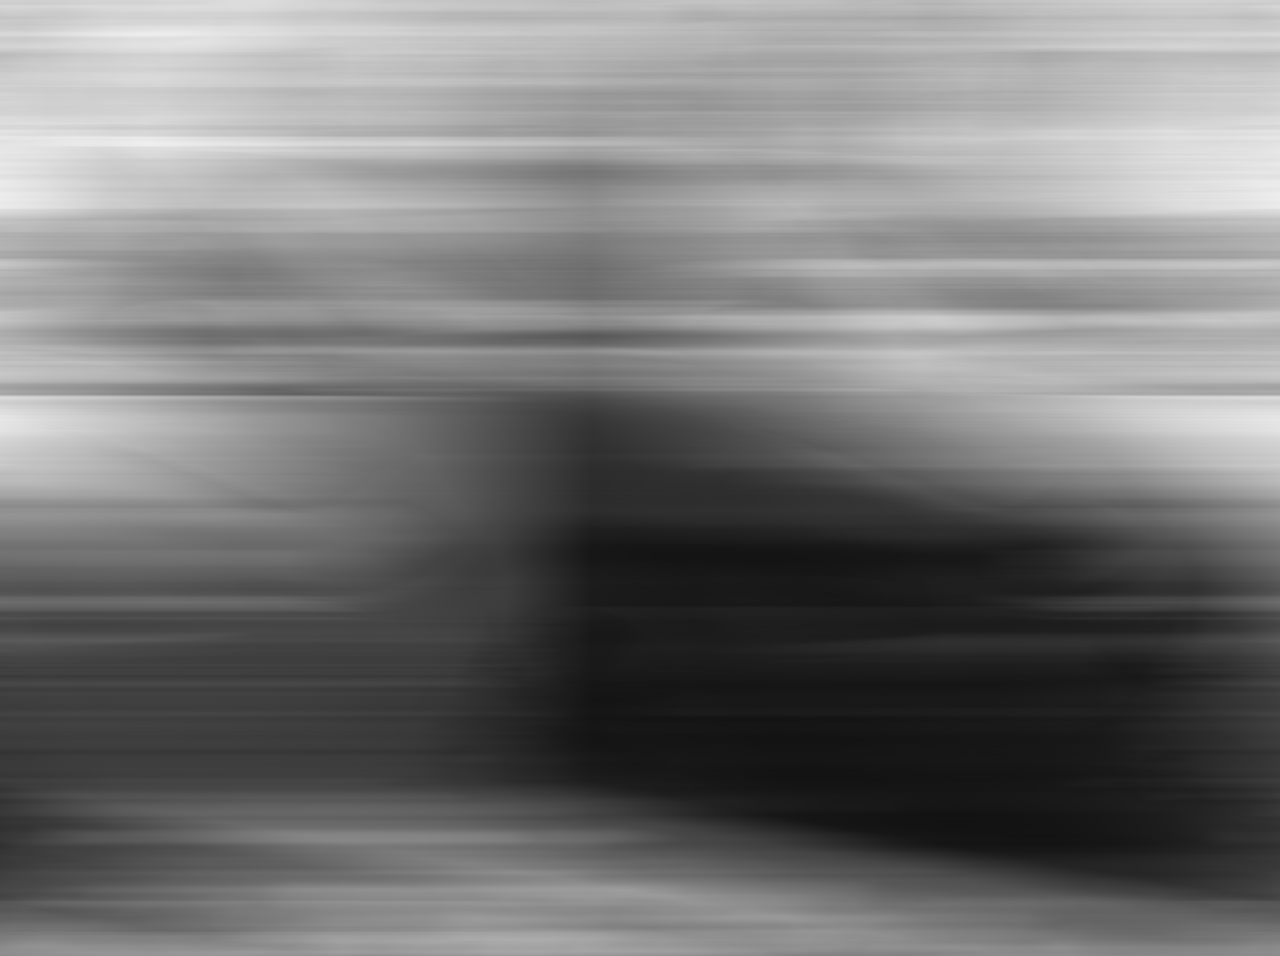
\includegraphics[scale=0.16]{G:/Study/tex_diploma/Pictures/fig3.png}
            \label{Fig3}
            \caption[Смаз при $k$ = 592]{Смаз при $k$ = 592}
        \end{figure}
\end{minipage}
\begin{minipage}{80mm}
  \begin{figure}[H]
            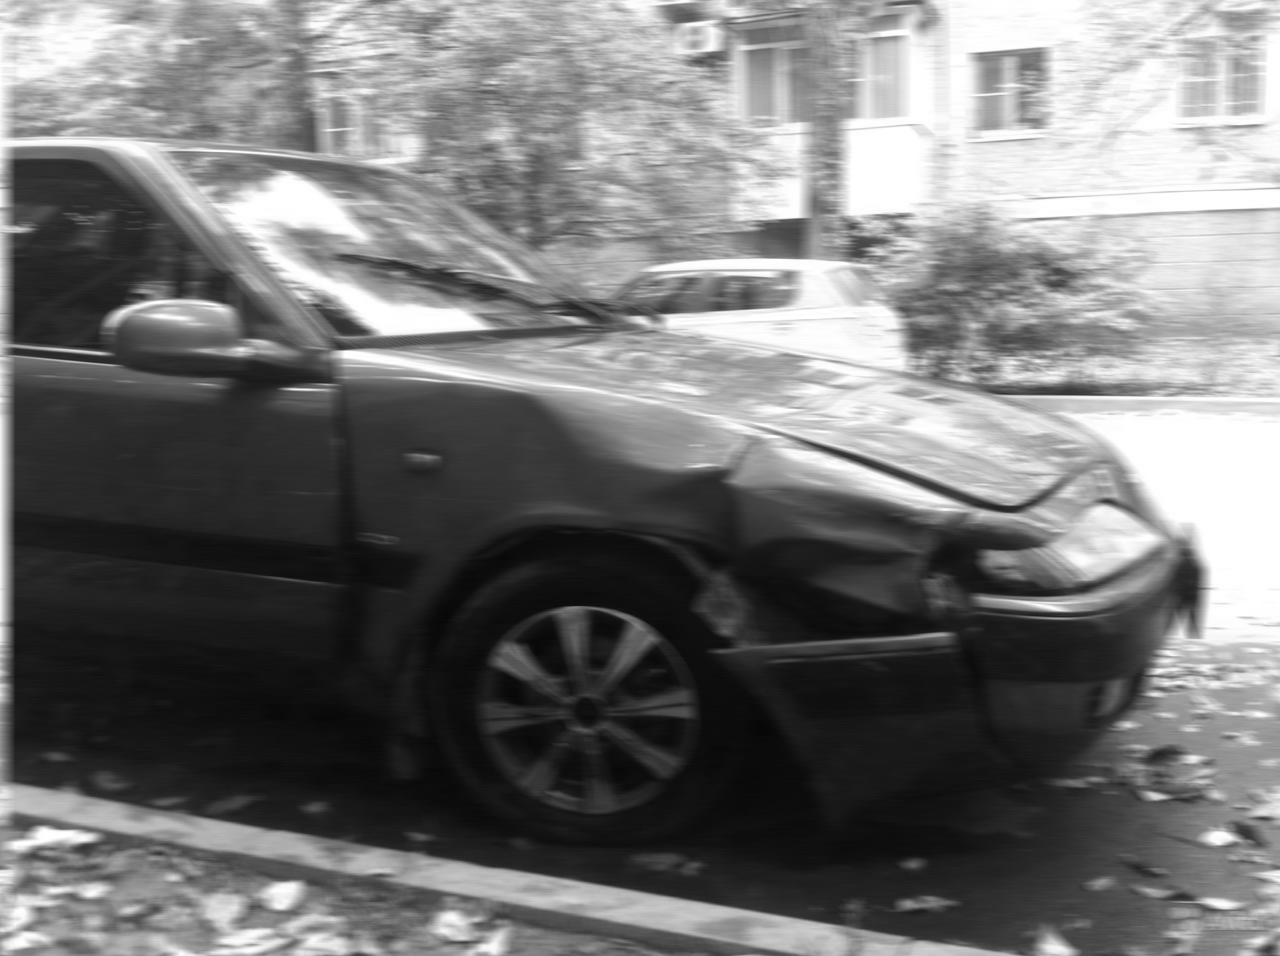
\includegraphics[scale=0.16]{G:/Study/tex_diploma/Pictures/fig4.png}
            \label{Fig4}
            \caption[Улучшенное фото]{Улучшенное фото}
        \end{figure}
\end{minipage}
\hfill

\end{example}
\vspace*{10mm}
\begin{example}

Второй пример показывает, что метод действительно работает плохо для 8-битных изображений. Однако, стоит отметить, что даже такой результат может оказаться достаточным, так как границы объектов вырисовываются достаточно четко.

\hspace*{-\parindent}
\begin{minipage}{80mm}
    \begin{figure}[H]
            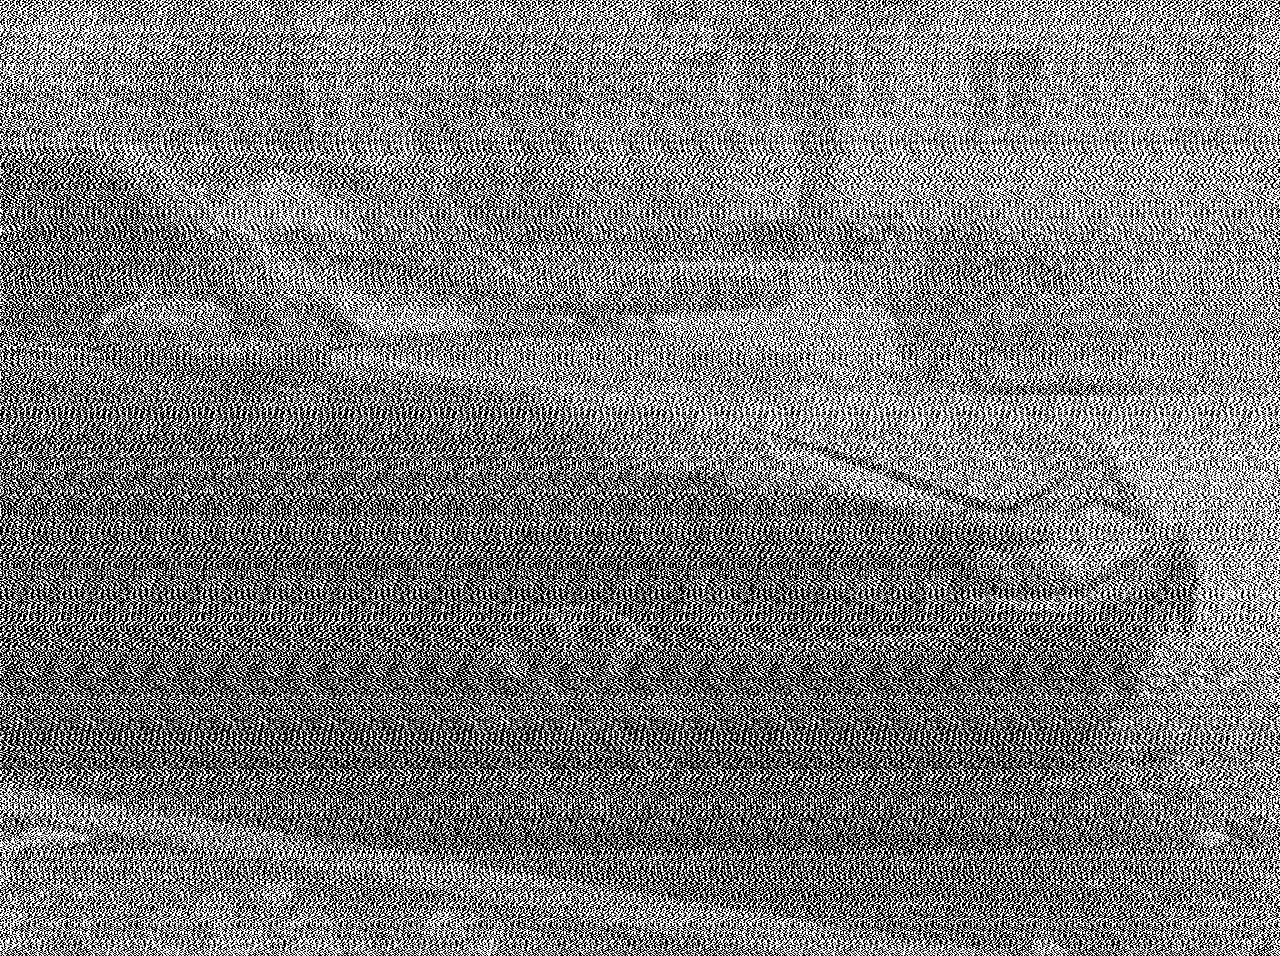
\includegraphics[scale=0.16]{G:/Study/tex_diploma/Pictures/fig5.png}
            \label{Fig3}
            \caption[Улучшение при $d$ = 2, $k$~=~242]{Улучшение при $d$ = 2, $k$~=~242}
        \end{figure}
\end{minipage}
\begin{minipage}{80mm}
  \begin{figure}[H]
            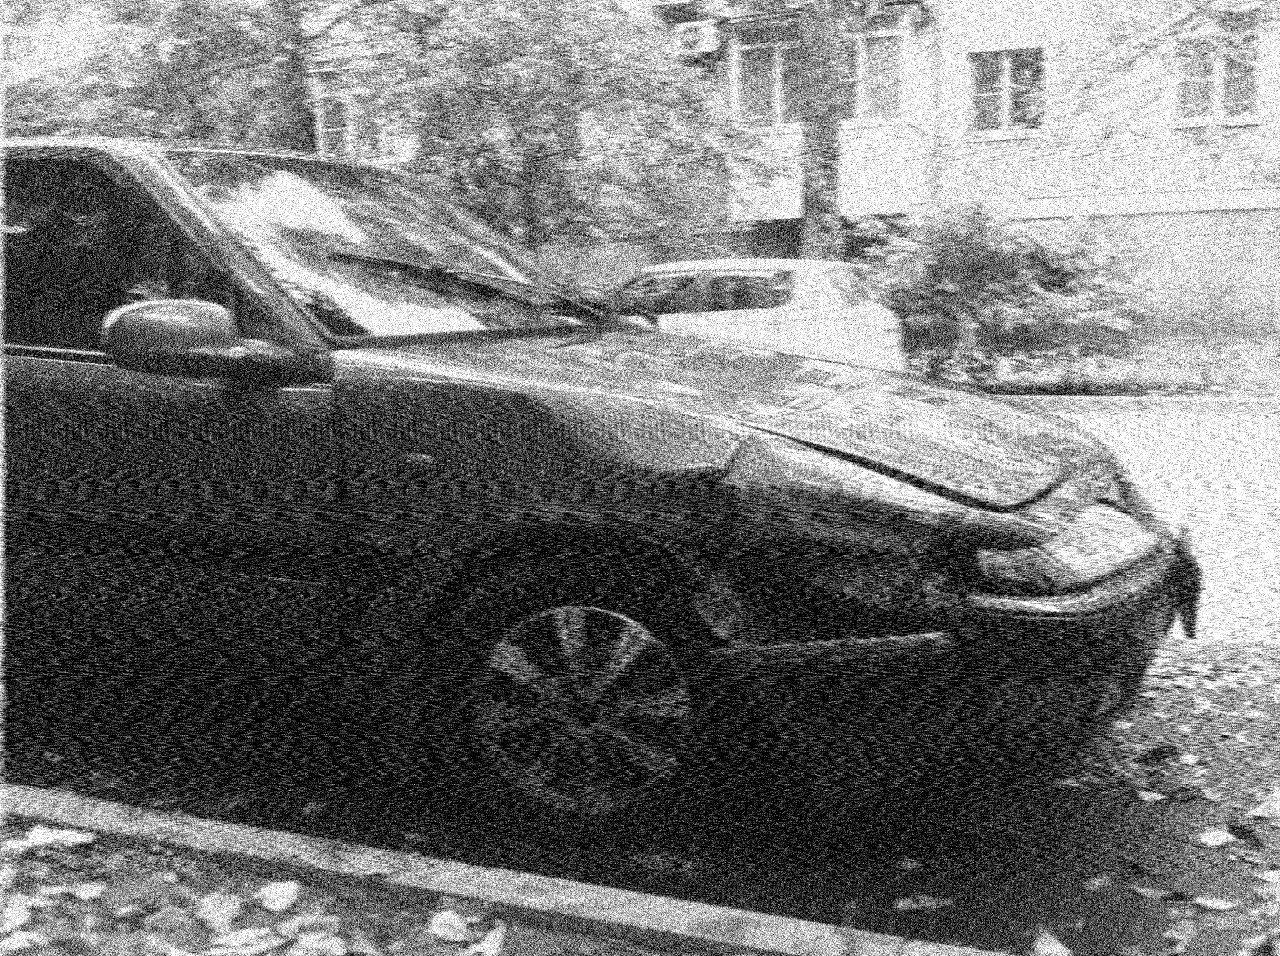
\includegraphics[scale=0.16]{G:/Study/tex_diploma/Pictures/fig6.png}
            \label{Fig4}
            \caption[Улучшение при $d$ = 8, $k$~=~248]{Улучшение при $d$ = 8, $k$~=~248}
        \end{figure}
\end{minipage}
\hfill

\vspace*{5mm}


Также этот пример иллюстрирует характер поведения результата в зависимости от параметра - чем больше $d$, тем более смазан оказывается результат, но с другой стороны, меньшее $d$ не позволяет нивелировать недостатки 8-битного невырожденного восстановления из-за большей размерности ``подизображений'' (так как число обусловленности для соответствующей матрицы смаза будет больше (\cite{cond}), а следовательно, и погрешность вычислений). Из этого следует вывод, что данный метод работает лучше при больших $d$.

\end{example}


%--------------------------------------
    \newpage
%-------------------------------------


    \section{Метод минимизации погрешности}

    \subsection{Описание проблемы}


    Больший интерес представляют методы, которые позволяют избавиться от смаза полностью. Учитывая специфику уравнения смаза $XC = S$, где~$X$~-~исходное~изображение, $C$~-~матрица~смаза и~$S$~-~смазанное~изображение, получим, что для идеального математически восстановления необходимо найти обратную к $C$ матрицу и домножить на нее справа. Конечно, на практике это либо дает плохой результат (случай невырожденного смаза), либо невозможно (случай вырожденного смаза) в силу особенностей задачи, а именно, матрицы смаза.


\begin{example}

Данный пример иллюстрирует, что необходимость в улучшении обычного восстановления для случая 8-битных входных данных действительно имеется даже для невырожденного случая. Здесь число смаза равно 491, то есть является простым числом, следовательно, смаз невырожденный.

\hspace*{-\parindent}
\begin{minipage}{80mm}
    \begin{figure}[H]
            \includegraphics[scale=0.07]{G:/Study/tex_diploma/Pictures/fig7.png}
            \label{Fig3}
            \caption[Восстановление 16-битного входа]{Восстановление

 16-битного входа}
        \end{figure}
\end{minipage}
\begin{minipage}{80mm}
  \begin{figure}[H]
            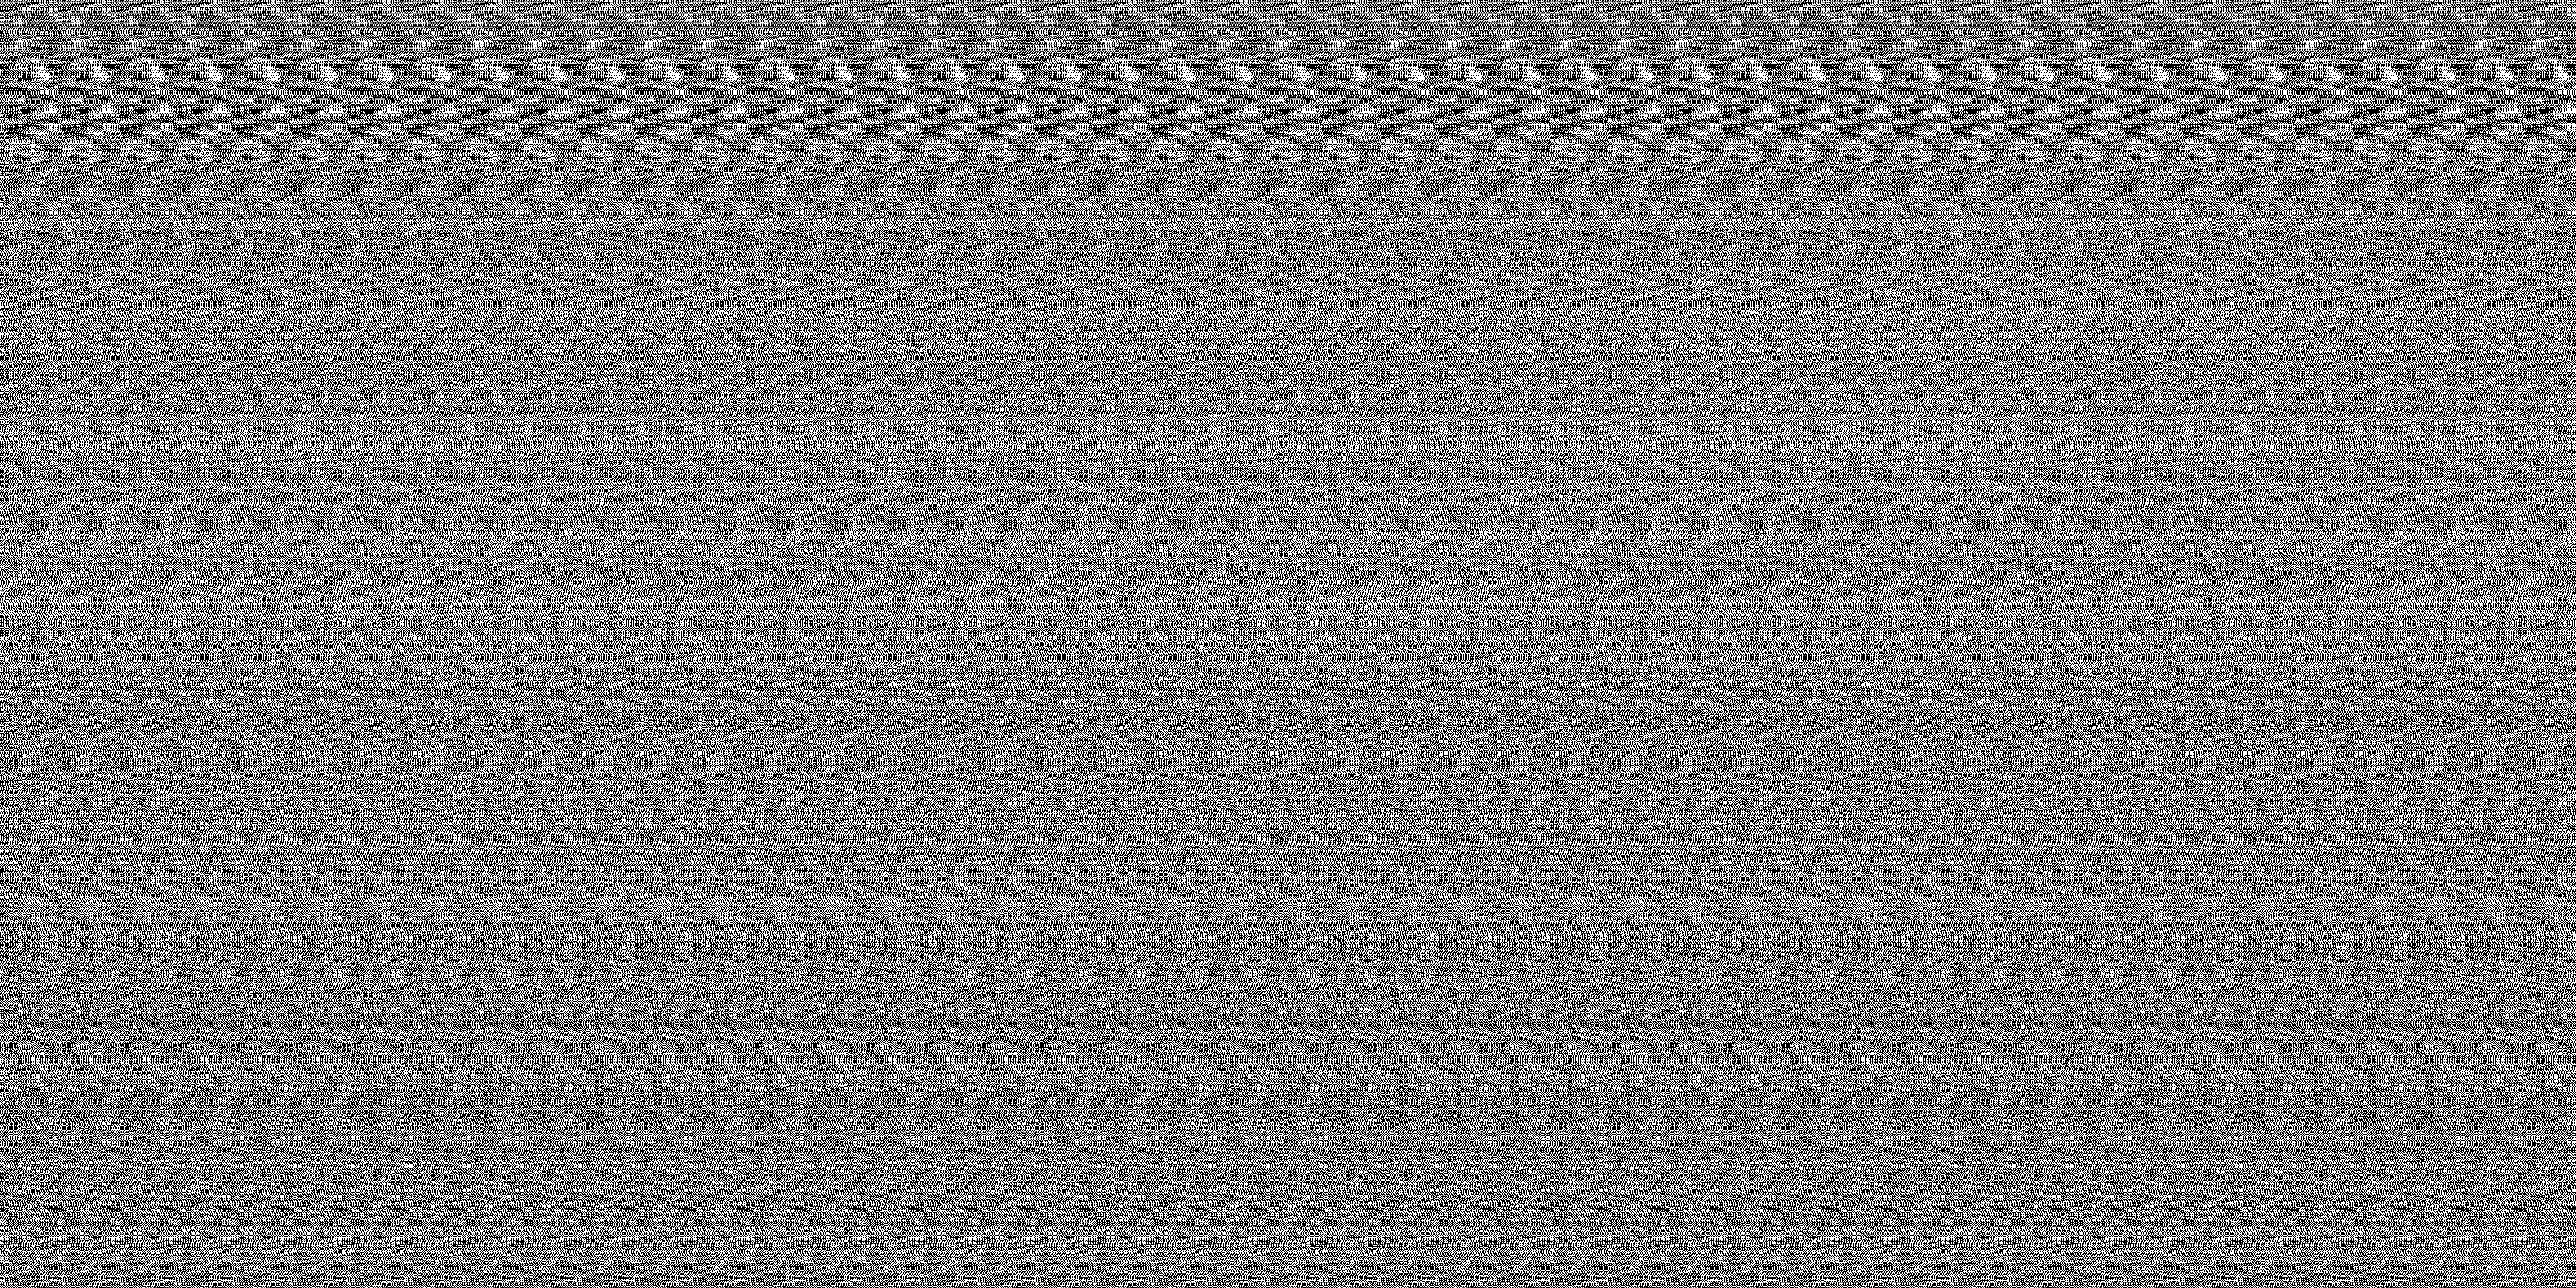
\includegraphics[scale=0.07]{G:/Study/tex_diploma/Pictures/fig8.png}
            \label{Fig4}
            \caption[Восстановление 8-битного~входа]{Восстановление

8-битного~входа}
        \end{figure}
\end{minipage}
\hfill
\end{example}
\vspace*{2mm}


    Первым препятствием является тот факт, что матрица смаза необратима при НОД$(n, k) \neq 1$, где $k$~-~число~смаза. Это означает, что в этом случае мы можем получить только приближенно-обратную матрицу, то есть такую матрицу $\tilde{C}$, что $C\tilde{C}$ наиболее близка по структуре к единичной (максимально близкие к единице числа на главной диагонали, к нулю в остальных местах). Объясняется это тем, что у вырожденной матрицы имеются собственные значения, равные нулю, а рассматривать $C$ и $\tilde{C}$ это все равно, что рассматривать их соответствующие матрицы $D$ и $\tilde{D}$, где $C = FDF^{-1},$ $\tilde{C} = F\tilde{D}F^{-1}$, и произведение нуля с чем угодно останется нулем.


    Вторым ограничением является формат данных, с которым приходится работать при обработке изображений. В момент получения кадра изображение оцифровывается и некоторая информация теряется (чем больше число смаза и чем меньше количество бит на пиксел при оцифровке, тем больше потери). Таким образом, уже на данном этапе происхоит потеря данных за счет погрешности округления.


    Имея в виду вышесказанное, необходимо сконструировать матрицу так, что при умножении на матрицу смаза справа она дает приближение единичной матрицы~---~это даст сохранение результата, максимально приближенного к исходному теоретически, а также учесть уже имеющуюся погрешность округления и минимизировать погрешность вычислений.


    \subsection{Возможные пути решения}


    Известно, что матрица смаза представима в виде $C = FDF^{-1}$, где $D$~-~диагональная матрица, причем на диагонали~-~собственные числа матрицы $C$, а $F$~-~дискретное преобразование Фурье соотвтетствующего размера. Понятно, что в случае, когда матрица полного ранга, ее обратная находится обращением всех чисел на диагонали. Известно, что обычный инверсный способ (\cite{model_proc}) может быть улучшен путем добавления регуляризационного фактора (\cite{addition}). Будем действовать по этому принципу с учетом специфики нашей задачи, тогда:


    \begin{list}{\arabic{qcounter})~}{\usecounter{qcounter}}
        \item Необратимость будем устранять заменой нулевых собственных чисел на некоторые числа с фиксированным модулем (модуль, так как собственные числа являются комплексными);
        \item Погрешность вычислений минизируем тем же способом~-~к ненулевым собственным числам, которые сильно малы по модулю, прибавим случайное комплексное число с тем же фиксированным модулем;
        \item Кроме того, оставшиеся достаточно малые собственные числа домножим так, чтобы по модулю они были равны фиксированному числу.
    \end{list}



    После соответствующих опреаций мы получим вместо матрицы $D^{-1}$, которая, вообще говоря, не всегда существует, некоторую матрицу $\tilde{D}$ такую, что $D\tilde{D} \approx E$ и $\tilde{C} = F\tilde{D}F^{-1}$. Рассмотрим, каким образом эти два преобразования повлияют на результат в теории и на практике. Эти результаты будут отличаться не только потому, что в реальной проблеме существуют погрешности, но так же и в силу особенностей порядка операций.


    \subsection{Особенности реализации на практике}


    В теории исходная матрица $X$ восстанавливается следующим порядком действий:

    $$S  F\tilde{D}F^{-1} = (X FDF^{-1}) F\tilde{D}F^{-1} = X FD\tilde{D}F^{-1},$$ то есть в идеализированной модели результат будет зависеть от того, насколько полученные числа на диагонали будут близки к числам, обратным к собственным. Также отдельно стоит отметить нулевые собственные числа - на что бы их не умножили, они останутся нулями, и соотвтествующие подобранные значения в матрице $\tilde{D}$ никакой роли не сыграют. На практике все выглядит немного иначе, поскольку матрица $S$ не расщепляется на составные части. Таким образом, влияние чисел, соответствующих нулевым собственным значениям, оказывается вполне реальным, поскольку итоговое приближение исходной матрицы $X$ будет выглядеть не иначе как $S (F\tilde{D}F^{-1}) = S\tilde{C}$. Соответственно, необходимо учитывать и этот фактор.


    \subsubsection{Поправка по умножению}


    Рассмотрим случай, когда сильно малых собственных значений не наблюдается. Тогда для каждого из них будет существовать некая поправка по умножению $\delta_i, i = \overline{0, n-1}$, а поправка по сложению не влияет на конечный результат. Это позвоялет нам рассматривать данный случай так же, как в теории, где внутренние преобразования Фурье взаимоуничтожаются. Обозначим $\tilde{E} = D\tilde{D}$, тогда:


    $$X = S \tilde{C} = X F\tilde{E}F^{-1},~~
    \tilde{E} = \begin{pmatrix}
          \frac{d_0}{d_0\delta_0} \hspace*{2mm} 0 \hspace*{4mm} \ldots \hspace*{10mm} 0 \\
          \hspace*{2mm} 0 \hspace*{2mm} \frac{d_1}{d_1\delta_1} \hspace*{2mm} \ldots \hspace*{10mm} 0 \\
          \ldots \hspace*{2mm} \ldots \hspace*{2mm} \ddots \hspace*{3mm} \ldots \\
          0 \hspace*{4mm} 0 \hspace*{2mm} \ldots \hspace*{2mm} \frac{d_{n-1}}{d_{n-1}\delta_{n-1}}
        \end{pmatrix} = \begin{pmatrix}
          \delta_0^{-1} \hspace*{5mm} 0 \hspace*{2mm} \ldots \hspace*{6mm} 0 \\
          \hspace*{2mm} 0 \hspace*{5mm} \delta_1^{-1} \hspace*{1mm} \ldots \hspace*{6mm} 0 \\
          \ldots \hspace*{2mm} \ldots \hspace*{2mm} \ddots \hspace*{3mm} \ldots \\
          0 \hspace*{4mm} 0 \hspace*{2mm} \ldots \hspace*{5mm} \delta_{n-1}^{-1}
        \end{pmatrix},
    $$ где $d$ - вектор собственных чисел матрицы $C$.


    Обозначим получившуюся матрицу $R = F\tilde{E}F^{-1}$. Тогда\\$R_{ij} = \frac{1}{n}\Sigma_{k=0}^{n-1} \delta_k^{-1} \xi^{(j-i)k}$, где $\xi$ есть первый корень из единицы степени $n$  $(e^{\frac{2\pi}{n}})$. Получим, что диагональные элементы $R$ равны между собой и равняются среднему величин обратных к поправкам по умножению, а элементы вне диагонали есть взвешенные средние $n$ различных корней из единицы. Важным замечением является тот факт, что эти корни различны для элементов на разных диагоналях, поскольку при удалении от главной диагонали угол между сосденими корнями $(\xi^{(j-i)k}$ и $\xi^{(j-i)(k+1)})$ увеличивается, и, соответственно, различные симметричные свойства теряются. Например, на первой диагонали, которая находится выше главной, ``базовый'' корень есть не что иное, как $\xi$, и, чтобы минимизировать элементы на этой диагонали, необходимо, чтобы вторая половина вектора поправок по умножению в точности повторяла первую ($\delta_0 = \delta_{\floor{\frac{n-1}{2}}+1}, \delta_1 = \delta_{\floor{\frac{n-1}{2}}+2}$ и т.д.), тогда как уже на второй диагонали условие для минимизации меняется на $\delta_i = -\delta_{\floor{\frac{n-1}{2}}+i+1}$. Таким образом, объединить условия для разных диагоналей не представляется возможным, даже если использовать поправки только для малого количества собственных значений. Это означает, что поправки по умножению, несмотря на то, что имеют детерминистскую природу, не позволяют достичь хороших результатов (кроме, конечно, случая, когда $\delta_i = \delta_j~ \forall~ i, j\in \overline{0, n-1}$, о нем пойдет речь в следующем пункте).


\hspace*{-\parindent}
\begin{minipage}{80mm}
    \begin{figure}[H]
            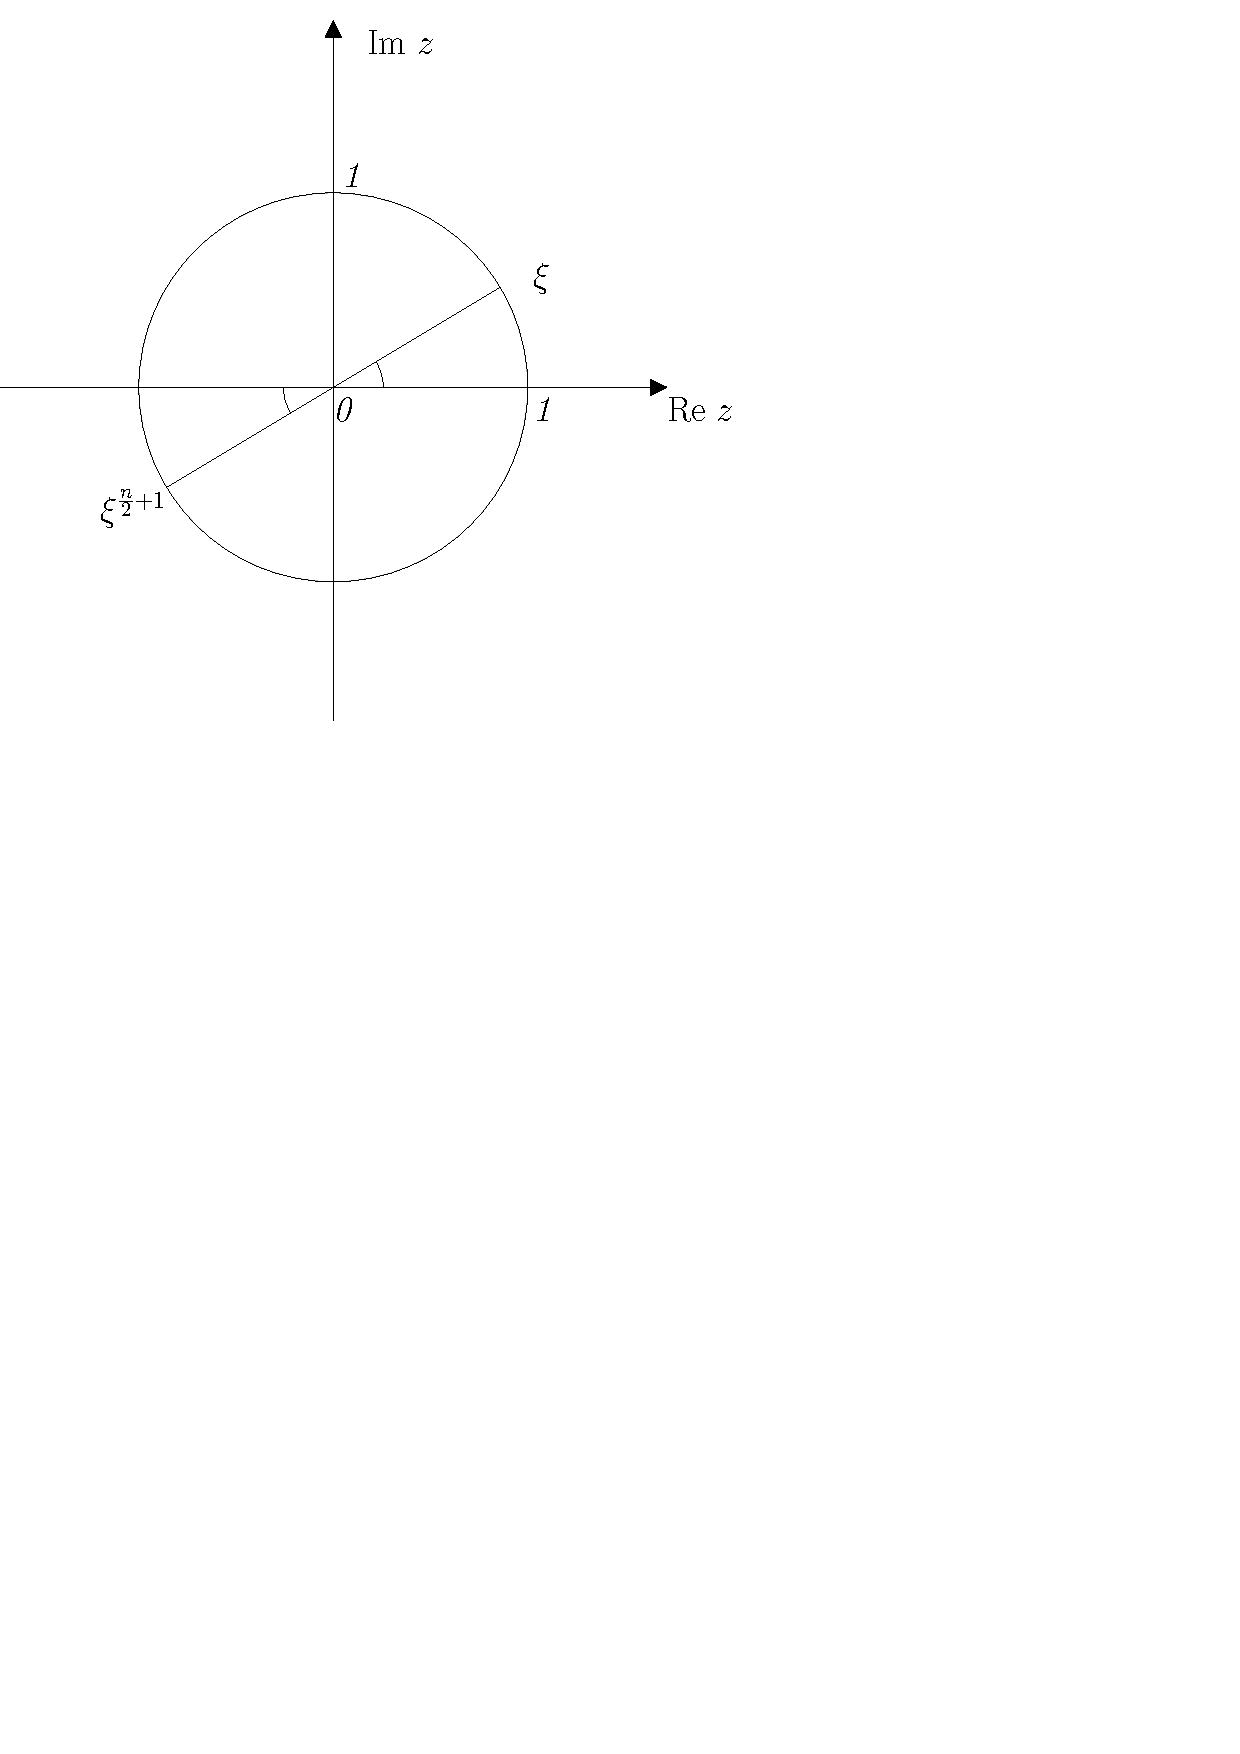
\includegraphics[scale=0.6]{G:/Study/tex_diploma/Pictures/graph1.pdf}
            \label{Graph1}
            \caption[Значения на первой диагонали после главной]{Значения на первой диагонали после главной}
        \end{figure}
\end{minipage}
\begin{minipage}{80mm}
  \begin{figure}[H]
            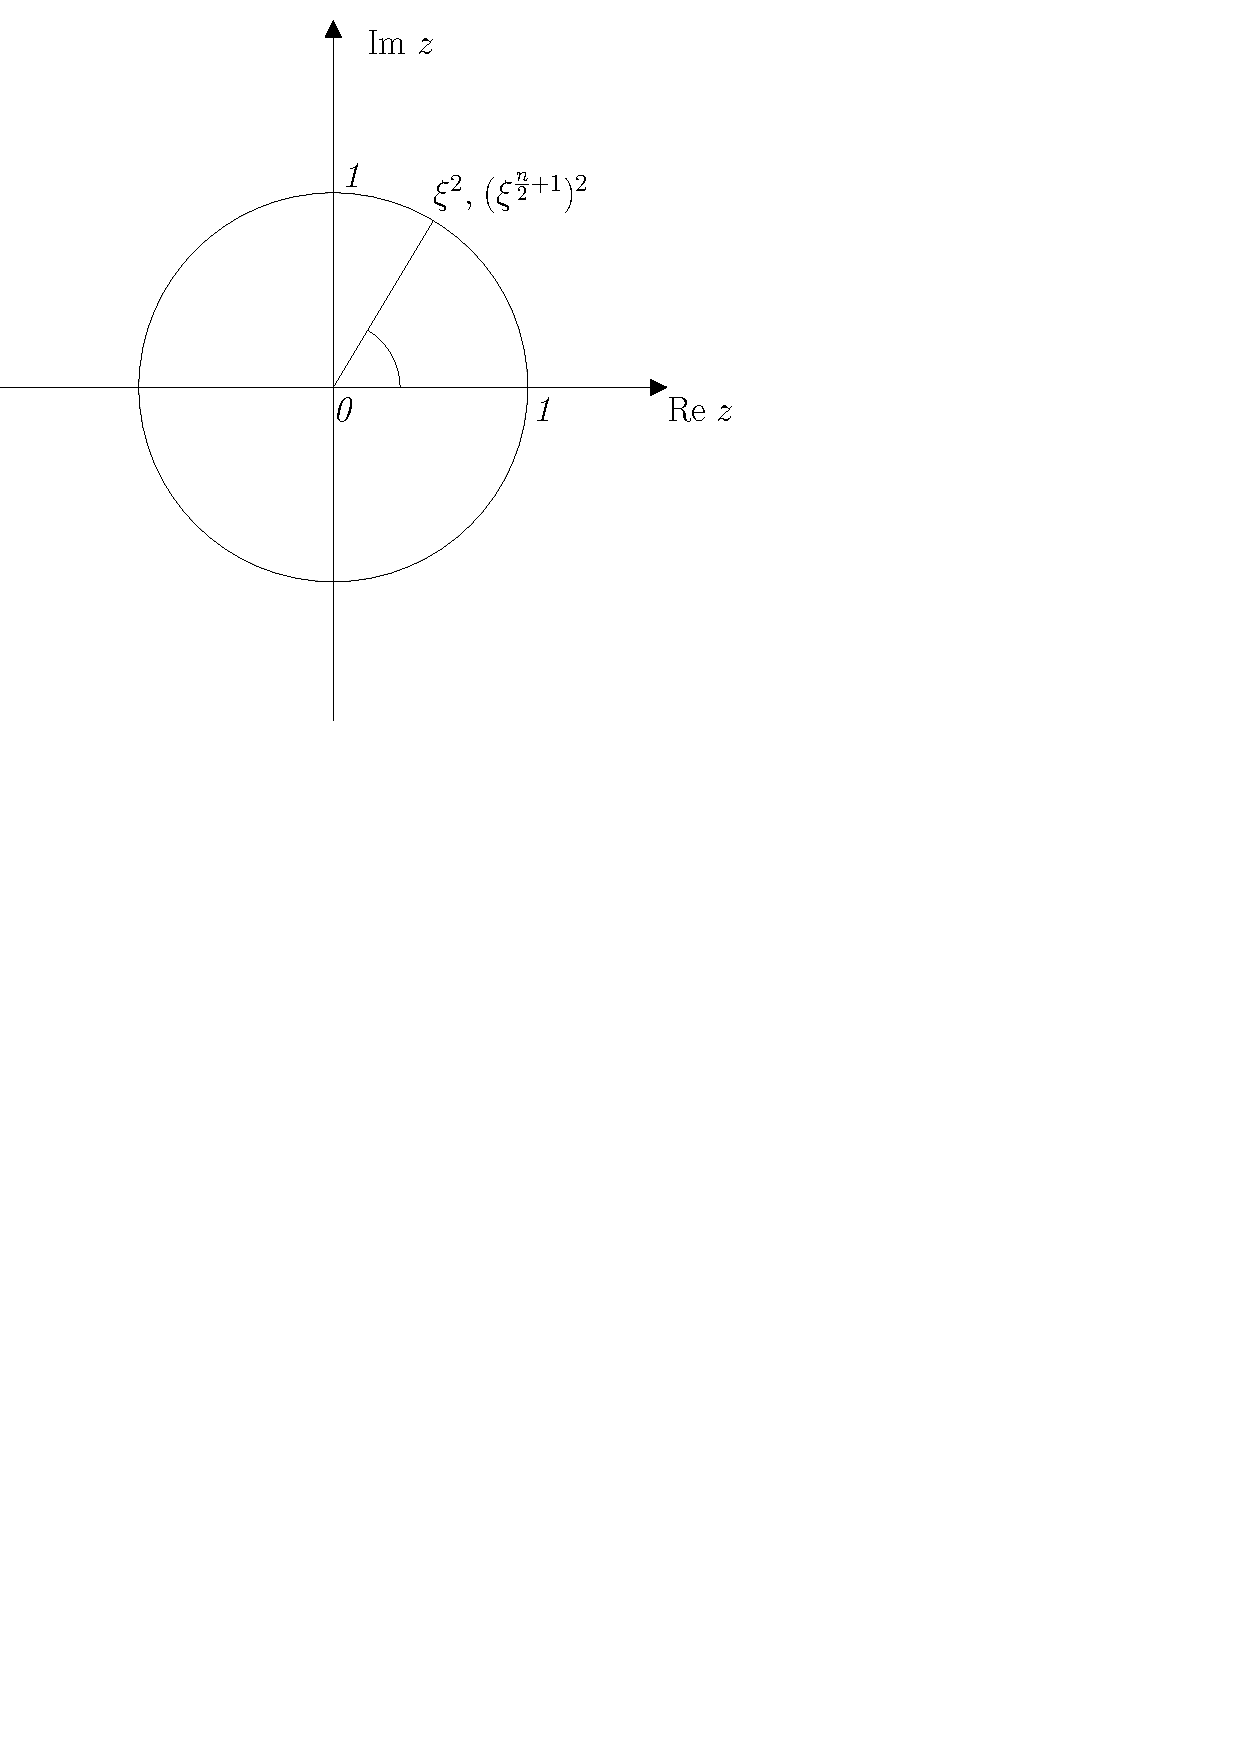
\includegraphics[scale=0.6]{G:/Study/tex_diploma/Pictures/graph2.pdf}
            \label{Graph2}
            \caption[Значения на второй диагонали после главной]{Значения на второй диагонали после главной}
        \end{figure}
\end{minipage}
\hfill
\vspace*{2mm}


    \subsubsection{Поправка по сложению}


    С поправкой по сложению все иначе. В теоретическом представлении задачи она позволяет лишь только осуществить псевдообращение матрицы смаза, но сами числа, которые мы прибавим, никоим образом не повлияют на результат. Следовательно, необходимо рассматривать матрицу

$\tilde{D}~=~diag(\frac{1}{d_0~+~\sigma_0},~\frac{1}{d_1~+~\sigma_1},~...,~\frac{1}{d_{n-1}~+~\sigma_{n-1}})$, где $\sigma$ - вектор значений поправки по сложению. Тогда аналогично п.3.3.1, положив $\gamma_i = d_i + \sigma_i$, $\tilde{R} = F\tilde{D}F^{-1}$, получим, что $\tilde{R}_{ij} = \frac{1}{n}\Sigma_{k=0}^{n-1} \gamma_k^{-1} \xi^{(j-i)k}$. Из уже приведенных рассуждений известно, что подбор для каждой отдельной диагонали не имеет смысла, соотвтественно, необходимо использовать новый подход. Так как для поправки по сложению мы отбираем числа с модулем, близким к или равным нулю, то соответствующие ``обратные'' собственные числа оказываются очень велики по модулю. Конечно, этого следует избегать, поскольку и так имеющаяся погрешность будет дополнительно усилена погрешностью вычислений. Поэтому, учитывая специфику поведения $R_{ij}$, перспективной выглядит идея установить для чисел $d_i$, которые попадают под условие на поправку по сложению, соответствующее $\sigma_i$ сделать фиксированным числом для любого такого $d_i$. Тогда, так как для каждого собственного числа на первой диагонали после главной имеется пара, то и на последующих диагоналях найдутся пары для новых чисел, которые взаимоуничтожатся при равных коэффициентах перед ними.  Тем не менее, поскольку поправка применяется не ко всем, а только к малым по модулю числам, некое подобие структуры, присущей исходной матрице, остается, и за счет этого восстановление остается возможным с теоретической точки зрения (теряются не все свойства матрицы).


    Действительно, оказывается, именно такой подход, единственный математически оправданный, является удачным и позволяет найти баланс между теоретической точностью и практической минимизацией погрешности. Примеры так же показывают, что для достижения этих результатов подойдет не только некая константа для всего вектора, но так же случайные комплексные числа с фиксированным модулем, причем постоянство модуля является определяющим свойством системы.


\subsubsection{Сравнение поправок на практике}


\begin{example} \label{ex32}

Все численные эксперименты, кроме данного примера, проведены на изображениях с серой цветовой гаммой, но, конечно, перенести алгоритм на цветные изображения очень просто. Здесь показано, каким образом влияют применение обеих поправок одновременно, то есть таким образом, что самые малые собственные значения получают поправку по сложению, а оставшиеся среди малых - поправку по умножению. Здесь показано восстановление 8-битного изображения.

\hspace*{-\parindent}
\begin{minipage}{80mm}
    \begin{figure}[H]
            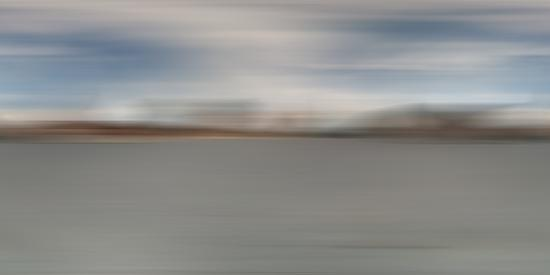
\includegraphics[scale=0.39]{G:/Study/tex_diploma/Pictures/fig12.jpg}
            \label{Pic12}
            \caption[Смазанное\\изображение]{Смазанное\\изображение}
        \end{figure}
\end{minipage}
\begin{minipage}{80mm}
    \begin{figure}[H]
            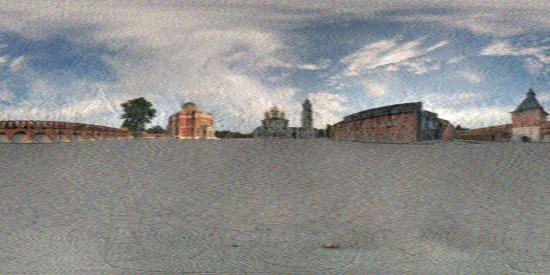
\includegraphics[scale=0.39]{G:/Study/tex_diploma/Pictures/fig13.jpg}
            \label{Pic13}
            \caption[Восстановление\\с поправкой]{Восстановление\\с поправкой}
        \end{figure}
\end{minipage}

\end{example}


\begin{example}

Данное восстановленное 16-битное фото показывает, что изменение части ``обратных'' собственных чисел при помощи поправки дает худший результат, чем восстановление без поправок, тем самым подвтерждая, что математическая (теоретическая) точность теряется.

\hspace*{-\parindent}
\begin{minipage}{80mm}
    \begin{figure}[H]
            \includegraphics[scale=0.07]{G:/Study/tex_diploma/Pictures/fig9.png}
            \label{Pic9}
            \caption[Восстановление\\с поправкой]{Восстановление\\с поправкой}
        \end{figure}
\end{minipage}
\begin{minipage}{85mm}
    \begin{figure}[H]
            \includegraphics[scale=0.07]{G:/Study/tex_diploma/Pictures/fig11.png}
            \label{Pic11}
            \caption[Восстановление\\без поправки]{Восстановление\\без поправки}
        \end{figure}
\end{minipage}
\vspace*{2mm}

\end{example}


На самом деле, этот эффект достигается не в любом случае --- известно (\cite{cond}), что для изображений с разрешением 4K это уже неверно из-за еще большего числа обусловленности матрицы смаза, и потери даже при 16-битной оцифровке не позволяют восстановить невырожденный смаз без видимого шума. Но для данного изображения (с разрешением 2K), как видно, это верно, и для того, чтобы убедиться в потере математической точности, этого достаточно.

\newpage

\begin{example}

Этот пример, как и Пример \autoref{ex32}, иллюстрирует восстановление на примере 8-битного изображения. Однако здесь используется поправка только по сложению, и можно сделать вывод, что ее достаточно для получения эффективного восстановления методом. Видно, что математическая точность пострадала ввиду изменения структуры матрицы путем изменения собственных значений, но, тем не менее, большая часть различимых деталей видна, что явялется следствием минимизации погрешности.

\hspace*{-\parindent}
\begin{minipage}{150mm}
  \begin{figure}[H]
            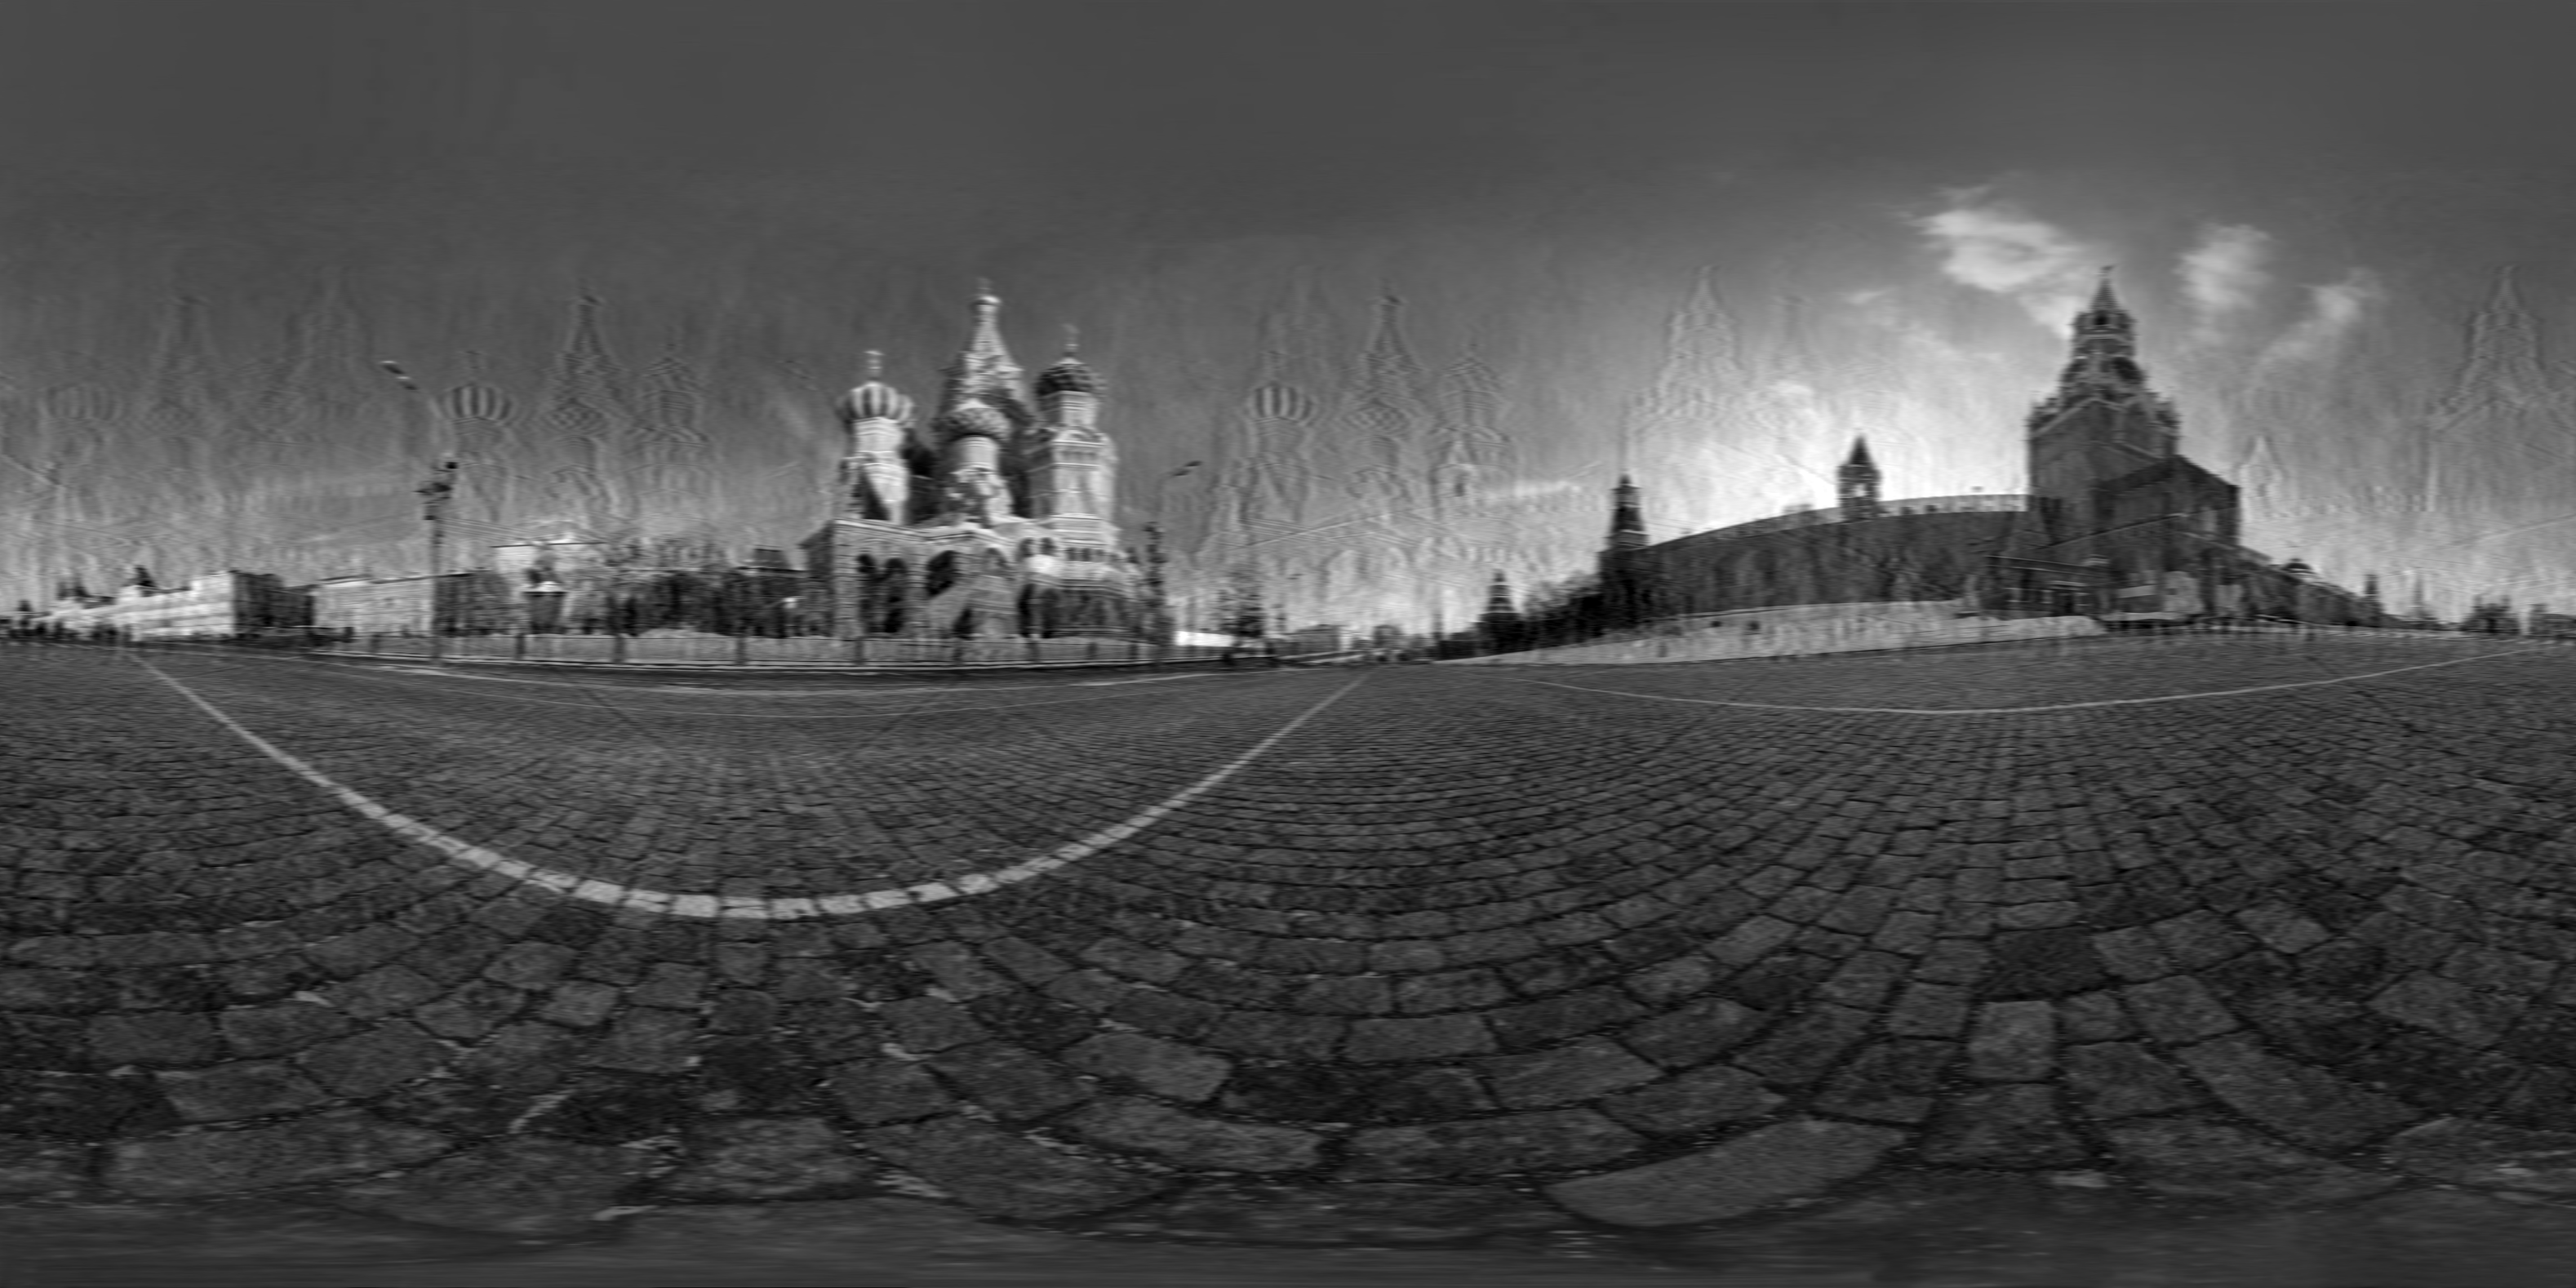
\includegraphics[scale=0.14]{G:/Study/tex_diploma/Pictures/fig10.png}
            \label{Pic10}
            \caption[Восстановление с применением поправки по сложению]{Восстановление с применением поправки по сложению}
        \end{figure}
\end{minipage}
\hfill
\vspace*{2mm}

\end{example}


Необходимо отметить, что в случае использования поправки по сложению оба типа изображений дают практически или совсем одинаковые результаты. Это говорит о том, что погрешность вычислений действительно удалось устранить или минимизировать, что лишний раз подтверждает приведенные выше рассуждения.



\newpage


\addcontentsline{toc}{section}{Список литературы}
\begin{thebibliography}{9}
\bibitem{blur_def}
Грузман И.С. Цифровая обработка изображений в информационных системах. / И.С.~Грузман, В.С.~Киричук, В.П.~Косых, Г.И.~Перетягин, А.А.~Спектор. Учебное пособие. --- Новосибисрк: Изд-во~НГТУ,~2002.~---~352~c.

\bibitem{kernel1}
Переславцева~Е.В. Двухфазная оценка ядра для устойчивого к ошибкам восстановления изображения, смазанного при движении. / Е.В.~Переславцева, М.В.~Филлипов. // Вестник МГТУ им. Н.Э. Баумана --- Сер.~``Приборостроение''~---~2012~---~C. 136-148.

\bibitem{kernel2}
Blind Deconvolution --- автоматическое восстановление смазанных изображений [Электронный ресурс]. --- Режим доступа https://habr.com/post/175717/. --- Заглавие с экрана. --- (Дата обращения - 12.06.2018).

\bibitem{model_proc}
Ежова К.В. Моделирование и обработка изображений. / К.В.~Ежова. Учебное пособие. --- СПб: НИУ ИТМО, 2011. --- 93 с.

\bibitem{matlab}
MATLAB Documentation [Электронный ресурс]. --- Режим доступа: https://www.mathworks.com/help/matlab/. --- Заглавие с экрана. --- (Дата обращения - 27.05.2018).

\bibitem{cond}
Козак А.В. Уравнение дискретной свертки с характеристической функцией сегмента и его приложение. / А.В. Козак, Б.Я. Штейнберг, О.Б. Штейнберг. Труды научной школы И.Б. Симоненко, выпуск второй. --- РнД: Издательство ЮФУ, 2015. --- 304 с.

\bibitem{fft_def}
Сергиенко А.Б. Цифровая обработка сигналов. / А.Б.~Сергиенко. --- СПб.: Питер, 2002. --- 608 с.

\bibitem{noise}
Сазонов В.В. Восстановление слабоконтрастных изображений. / В.В. Сазонов, М.А. Щербаков. // International Scientific Conference
``Advanced Information Technologies and Scientific Computing'' --- 2014 --- С. 343-346.

\bibitem{addition}
Дайнеко М.В. Восстановление смазанных под углом и зашумленных изображений без учета граничных условий. / М.В. Дайнеко, В.С. Сизиков. // Научно-технический вестник Санкт-Петербургского университета информационных технологий, механики и оптики --- 2010 --- №4(68) --- С. 28-32.

\end{thebibliography}


\end{document}






